%\newpage
\section{TÍNH ĐƠN ĐIỆU VÀ CỰC TRỊ CỦA HÀM SỐ}
\subsection{LÝ THUYẾT CẦN NHỚ}
\subsubsection{Tính đơn điệu của hàm số}
\indam{Định nghĩa:}
\begin{boxdn}
	Kí hiệu $K$ là khoảng hoặc đoạn hoặc nửa khoảng. Giả sử hàm số $y=f(x)$ xác định trên $K$.\\
	Hàm số $y=f(x)$ gọi là \textit{đồng biến (tăng)} trên $K$ nếu với mọi $x_1$, $x_2$ thuộc $K$ mà $x_1<x_2$ thì $f\left(x_1\right)<f\left(x_2\right)$.\\
	Hàm số $y=f(x)$ gọi là \textit{nghịch biến (giảm)} trên $K$ nếu với mọi $x_1$, $x_2$ thuộc $K$ mà $x_1<x_2$ thì $f\left(x_1\right)>f\left(x_2\right)$.\\
	Nếu hàm số $y=f(x)$ đồng biến trên $K$ thì đồ thị của nó {\textit{đi lên}} từ trái sang phải (Hình 1a).\\
	Nếu hàm số $y=f(x)$ nghịch biến trên $K$ thì đồ thị của nó {\it{đi xuống}} từ trái sang phải (Hình 1b).
	\begin{center}
		\begin{tikzpicture}[scale=0.7, font=\footnotesize, line join=round, line cap=round, >=stealth]
			\draw[->] (-1.5,0)--(4.5,0) node [below]{$x$};
			\draw[->] (0,-1.5)--(0,5) node [left]{$y$};
			\draw (3,0)node[below]{$K$} (2,-2)node{a)} (1.8,2.7)node[red]{$y=f(x)$};
			% \draw[smooth,red,samples=300,domain=1.5:4] plot(\x,{0.25*(\x)^2});
			\draw[red] (1.5,0.5)parabola (4,4);
			\fill (0,0)circle (1pt)node[below left]{$O$};
			\draw[dashed] (1.5,0)--(1.5,0.5625) (4,0)--(4,4);
			%===
			\draw[->] (6.5,0)--(12.5,0) node [below]{$x$};
			\draw[->] (8,-1.5)--(8,5) node [left]{$y$};
			\draw (11,0)node[below]{$K$} (10,-2)node{b)} (10.4,1.5)node[red]{$y=f(x)$};
			%\draw[smooth,red,samples=300,domain=9.3:12] plot(\x,{-0.25*(\x)^2+4*(\x)-11.5});
			\draw[red] (9.3,4.0775) parabola (12,0.5);
			\fill (8,0)circle (1pt)node[below left]{$O$};
			\draw[dashed] (9.3,0)--(9.3,4.0775) (12,0)--(12,0.5);
			\draw (5.5,-3)node{Hình 1};
		\end{tikzpicture}
	\end{center}
	Hàm số đồng biến hoặc nghịch biến trên $K$ được gọi chung là \textit{đơn điệu} trên $K$.
\end{boxdn}
\begin{dl}
	Cho hàm số $y=f(x)$ có đạo hàm trên $K$.\\
	Nếu $f'(x)>0$ với mọi $x$ thuộc $K$ thì hàm số $y=f(x)$ đồng biến trên $K$.\\
	Nếu $f'(x)<0$ với mọi $x$ thuộc $K$ thì hàm số $y=f(x)$ nghịch biến trên $K$.
\end{dl}
\begin{note}
	Khi xét tính đơn điệu của hàm số mà chưa cho khoảng $K$, ta hiểu xét tính đơn điệu của hàm số đó trên tập xác định của nó.	
\end{note}
\noindent Từ kết quả trên, để xét tính đơn điệu của hàm số $y=f(x)$, ta thực hiện các bước sau: \\
\textit{Bước 1.} Tìm tập xác định $\mathscr{D}$ của hàm số.\\
\textit{Bước 2.} Tính đạo hàm $f'(x)$ của hàm số. Tìm các điểm $x_1$; $x_2$;\ldots; $x_n$ thuộc $\mathscr{D}$ mà tại đó đạo hàm $f'(x)$ bằng $0$ hoặc không tồn tại.\\
\textit{Bước 3.} Sắp xếp các điểm $x_1$; $x_2$;\ldots; $x_n$ theo thứ tự tăng dần, xét dấu $f'(x)$ và lập bảng biến thiên.\\
\textit{Bước 4.} Nêu kết luận về các khoảng đồng biến, nghịch biến của hàm số.
\begin{note}
	\begin{enumerate}
		\item Nếu hàm số $y=f(x)$ có đạo hàm trên $K$, $f'(x) \geq 0$ với mọi $x \in K$ và $f'(x)=0$ chỉ tại một số hữu hạn điểm thì hàm số đồng biến trên $K$.
		\item Nếu hàm số $y=f(x)$ có đạo hàm trên $K$, $f'(x) \leq 0$ với mọi $x \in K$ và $f'(x)=0$ chỉ tại một số hữu hạn điểm thì hàm số nghịch biến trên $K$.
	\end{enumerate}
\end{note}
\subsubsection{Cực trị của hàm số}
\indam{Định nghĩa:}
\begin{boxdn}
		\immini
		{
			Cho hàm số $y=f(x)$ xác định trên tập hợp $\mathscr{D}$ và $x_0 \in~ \mathscr{D}$.
			\begin{itemize}
				\item Nếu tồn tại một khoảng $(a;b)$ chứa điểm $x_0$ và $(a;b) \subset \mathscr{D}$ sao cho $f(x)<f\left(x_0\right)$ với mọi $x \in(a;b) \setminus\left\{x_0\right\}$ thì $x_0$ được gọi là một \textbf{điểm cực đại}, $f\left(x_0\right)$ được gọi là \textbf{giá trị cực đại} của hàm số $y=f(x)$, kí hiệu $y_{\text{CĐ}}$.
				\item Nếu tồn tại một khoảng $(a;b)$ chứa điểm $x_0$ và $(a;b) \subset \mathscr{D}$ sao cho $f(x)>f\left(x_0\right)$ với mọi $x \in(a;b) \setminus\left\{x_0\right\}$, thì $x_0$ được gọi là một \textbf{điểm cực tiểu}, $f\left(x_0\right)$ được gọi là \textbf{giá trị cực tiểu} của hàm số $y=f(x)$, kí hiệu $y_{\text{CT}}$.
			\end{itemize}
		}
		{
			\begin{tikzpicture}[scale=1, font=\footnotesize, line join=round, line cap=round, >=stealth]
				\def\xmin{-2} \def\xmax{6}
				\def\ymin{-1} \def\ymax{5} 
				\draw[->] (\xmin,0)--(\xmax,0) node [below]{$x$};
				\draw[->] (0,\ymin)--(0,\ymax) node [left]{$y$};
				\draw[red] (0.5,0.5) parabola bend  (1,2) (1.5,1.5)  parabola bend (2,1) (3,2.5) parabola bend (4,4) (4.5,3.5) parabola bend (5,3) (5.5,3.5)
				(4,4)node[above]{$y=f(x)$}
				;
				\draw[dashed] (1,0)--(1,2)--(0,2)
				(2,0)--(2,1)--(0,1)
				(4,0)--(4,4)--(0,4) (5,0)--(5,3)--(0,3); 
				\fill (1,0)circle(1pt)node[below]{$x_1$} (2,0)circle(1pt)node[below]{$x_2$}
				(4,0)circle(1pt)node[below]{$x_3$}
				(5,0)circle(1pt)node[below]{$x_4$}
				(1,2)circle(1pt)
				(2,1)circle(1pt)
				(4,4)circle(1pt)
				(5,3)circle(1pt)
				(0,0)circle(1pt)node[below left]{$O$}
				;
				\draw[orange,->] (2,-0.8)--(1.1,-0.4);
				\draw[orange,->] (2,-0.8)--(3.9,-0.4);
				\draw[blue,->] (4.5,-0.8)--(4.9,-0.4);
				\draw[blue,->] (4.5,-0.8)--(2.1,-0.4);
				\draw[orange,->] (-1,3)--(0,4);
				\draw[orange,->] (-1,3)--(0,2);
				\draw[blue,->] (-1,2)--(0,3);
				\draw[blue,->] (-1,2)--(0,1);
				\draw (2,-1) node{Điểm cực đại}
				(4.5,-1) node{Điểm cực tiểu} 
				(-1.7,3.3) node{Giá trị}
				(-1.7,2.8) node{cực đại}
				(-1.7,2.3) node{Giá trị}
				(-1.7,1.8) node{cực tiểu}
					;
			\end{tikzpicture}
		}		

\end{boxdn}
\begin{note}
	\begin{enumerate}
		\item Điểm cực đại và điểm cực tiểu được gọi chung là \textbf{điểm cực trị} của hàm số. Giá trị cực đại và giá trị cực tiểu được gọi chung là \textbf{giá trị cực trị} (còn gọi là {\bf{cực trị}}) của hàm số.
		\item Nếu $x_0$ là một điểm cực trị (điểm cực đại, điểm cực tiểu) của hàm số $y=f(x)$ thì ta cũng nói hàm số $y=f(x)$ đạt cực trị (cực đại, cực tiểu) tại $x_0$.
		\item Hàm số có thể đạt cực đại và cực tiểu tại nhiều điểm trên $\mathscr{D}$.
		\item Nếu $x_0$ là điểm cực trị của hàm số $y=f(x)$ thì điểm $M\left(x_0;f\left(x_0\right)\right)$ là một điểm cực trị của đồ thị hàm số $y=f(x)$.
	\end{enumerate}
\end{note}
\begin{dl}
	Cho hàm số $y=f(x)$ liên tục trên khoảng $(a; b)$ chứa điểm $x_0$ và có đạo hàm trên các khoảng $(a; x_0)$ và $(x_0; b)$. Khi đó
	\begin{itemize}
		\item Nếu $f'(x)<0$ với mọi $x\in (a; x_0)$ và $f'(x)>0$ với mọi $x\in (x_0; b)$ thì hàm số $y=f(x)$ đạt cực tiểu tại điểm $x_0$;
		\item Nếu $f'(x)>0$ với mọi $x\in (a; x_0)$ và $f'(x)<0$ với mọi $x\in (x_0; b)$ thì hàm số $y=f(x)$ đạt cực đại tại điểm $x_0$.
	\end{itemize}
\end{dl}
\begin{nx}
	Từ kết quả trên, đế tìm cực trị của hàm số $y=f(x)$, ta thực hiện như sau
	\begin{itemize}
		\item \textit{Bước 1.} Tìm tập xác định $\mathscr{D}$ của hàm số.
		\item \textit{Bước 2.} Tính đạo hàm $f'(x)$ của hàm số. Tìm các điểm $x_1$; $x_2$;\ldots; $x_n$ thuộc $\mathscr{D}$ mà tại đó đạo hàm $f'(x)$ bằng $0$ hoặc không tồn tại.
		\item \textit{Bước 3.} Xét dấu $f'(x)$. Nếu $f'(x)$ đổi dấu từ âm sang dương khi $x$ qua điểm $x_i$ $(i=1, 2, \ldots)$ thì hàm số đạt cực tiểu tại $x_i$. Nếu $f'(x)$ đổi dấu từ dương sang âm khi $x$ qua điểm $x_i$ $(i=1, 2, \ldots)$ thì hàm số đạt cực đại tại $x_i$.
	\end{itemize}
\end{nx}
\begin{note}
	\begin{enumerate}
		\item Nếu $f'(x)=0$ nhưng không đổi dấu khi $x$ qua điểm $x_i$ $(i=1, 2, \ldots)$ thì hàm số không có cực trị tại $x_i$.
		\item Nếu $f'(x)$ không đổi dấu trên khoảng $K$ thì $f(x)$ không có cực trị trên khoảng đó.
	\end{enumerate}
\end{note}

%-------------------------------------------------------------------------------------------------------------
\subsection{PHÂN LOẠI VÀ PHƯƠNG PHÁP GIẢI TOÁN}
\begin{dang}{Xác định tính đơn điệu của hàm số dựa vào đồ thị}
	{\bf{Phương pháp giải}}
	\begin{itemize}
		\item \textit{Bước 1.} Xác định khoảng đồng biến: Quan sát trên đồ thị, nếu đồ thị {\it{đi lên}} từ trái sang phải, đó là khoảng hàm số đồng biến. Ghi lại khoảng giá trị của $x$ tương ứng.
		\item \textit{Bước 2.} Xác định khoảng nghịch biến: Quan sát trên đồ thị, nếu đồ thị {\it{đi xuống}} từ trái sang phải, đó là khoảng hàm số nghịch biến. Ghi lại khoảng giá trị của $x$ tương ứng.		
	\end{itemize}
\end{dang}

\begin{vd}%[2D1N1-2]
\immini{Trong $8$ phút kể từ khi xuất phát, độ cao $h$ (tính bằng mét) của khinh khí cầu vào thời điểm $t$ phút được cho bởi công thức $h(t)=6t^3-81t^2+324t$. Đồ thị của hàm số $h(t)$ được biểu diễn trong hình bên. Trong các khoảng thời gian nào khinh khí cầu tăng dần độ cao, giảm dần độ cao? Độ cao của khinh khí cầu vào các thời điểm $3$ phút và $6$ phút sau khi xuất phát có gì đặc biệt?
}{
	\begin{tikzpicture}[scale=0.7, font=\footnotesize, line join=round, line cap=round, >=stealth]
		\def\xmin{-2} \def\xmax{9}
		\def\ymin{-1} \def\ymax{6} 
		\draw[->] (\xmin,0)--(\xmax,0) node [below]{$t$};
		\draw[->] (0,\ymin)--(0,\ymax) node [left]{$h$};
		\clip (\xmin+0.1,\ymin+0.1) rectangle (\xmax-0.1,\ymax-0.1);
		\draw[smooth,samples=300,domain=0:7.3,red] plot(\x,{0.07*(\x)^3-0.89*(\x)^2+3.39*(\x)});
		\fill (0,0)circle (1pt)node[below left]{$O$};
		\fill (0,3.35)circle(1pt )node[left]{$324$} (0,4.05)circle(1pt )node[left]{$405$} (0,4.6)circle(1pt )node[left]{$480$}
		(3,0)circle(1pt )node[below]{$3$}
		(5.6,0)circle(1pt )node[below]{$6$}
		(7.3,0)circle(1pt )node[below]{$8$}
		;
		\draw[dashed] (3,0)--(3,4.05)--(0,4.05) (5.6,0)--(5.6,3.35)--(0,3.35) (7.3,0)--(7.3,4.6)--(0,4.6);
		\fill (3,4.05)circle (1pt)
		(5.6,3.35)circle (1pt)
		(7.3,4.6)circle (1pt)
		;
	\end{tikzpicture}
}
\loigiai{
	\begin{itemize}
		\item Khinh khí cầu tăng độ cao (đồng biến) trong khoảng $(0;3)$ và $(6;8)$.
		\item Khinh khí cầu giảm độ cao (nghịch biến) trong khoảng $(3;6)$.
		\item Độ cao tại $t=3$ là $405$ (giá trị cực đại).
		\item Độ cao tại $t=6$ là $324$ (giá trị cực tiểu).
	\end{itemize}
}	
\end{vd}
\begin{vd}%[2D1N1-2]
	Tìm các khoảng đơn điệu của hàm số $y= f(x)$ có đồ thị cho ở hình vẽ.
	\begin{center}
		\begin{tikzpicture}[scale=0.7, font=\footnotesize, line join=round, line cap=round, >=stealth]
			\def\xmin{-3} \def\xmax{9}
			\def\ymin{-3} \def\ymax{5} 
			\draw[->] (\xmin,0)--(\xmax,0) node [below]{$x$};
			\draw[->] (0,\ymin)--(0,\ymax) node [left]{$y$};
			\clip (\xmin+0.1,\ymin+0.1) rectangle (\xmax-0.1,\ymax-0.1);
			\draw[red,smooth,samples=300,domain=-2:8] plot(\x,{0.06*(\x)^3-0.54*(\x)^2+0.9*(\x)+1.5});
			\fill (0,0)circle (1pt)node[below left]{$O$}
			(-2,0)circle (1pt)node[below left]{$-2$}
			(1,0)circle (1pt)node[below]{$1$}
			(5,0)circle (1pt)node[below]{$5$}
			(8,0)circle (1pt)node[below]{$8$}
			;
			\draw[dashed] (-2,0)--(-2,\ymin) (8,0)--(8,\ymax) (1,0)--(1,1.92);
			\fill (1,1.92)circle(1pt) ;
		\end{tikzpicture}
	\end{center}
	\loigiai{
		Hàm số đồng biến trên các khoảng $(-2;1)$ và $(5;8)$, nghịch biến trên khoảng $(1;5)$.
	}
\end{vd}

\begin{dang}{Xét tính đơn điệu của hàm số bằng công thức}
	{\bf{Phương pháp giải}}
	\begin{itemize}
		\item \textit{Bước 1.} Tìm tập xác định $\mathscr{D}$ của hàm số.
		\item \textit{Bước 2.} Tính đạo hàm $f'(x)$. Tìm các điểm mà tại đó $f'(x)=0$ hoặc $f'(x)$ không xác định.
		\item \textit{Bước 3.} Lập bảng biến thiên
		\begin{itemize}
			\item Sắp xếp các điểm tìm được ở Bước 2 theo thứ tự tăng dần trên trục số.
			\item Xác định dấu của $f'(x)$ trên mỗi khoảng bằng cách chọn một giá trị $x$ bất kỳ trong khoảng đó và thay vào $f'(x)$.
			\item Dựa vào dấu của $f'(x)$ vẽ mũi tên thể hiện chiều biến thiên của $f(x)$.
				\begin{itemize}
					\item $f'(x)>0$ suy ra mũi tên đi lên (đồng biến).
					\item $f'(x)<0$ suy ra mũi tên đi xuống (nghịch biến).
				\end{itemize}
			\item Kết luận về các khoảng đồng biến, nghịch biến.
		\end{itemize}
	\end{itemize}
\end{dang}

\begin{vd}%[TeX hóa SGK CTST 12]%[Phạm Tiến Long]%[2D1H1-2]
	Xét tính đơn điệu của các hàm số sau:
	\begin{multicols}{3}
		\begin{enumerate}
			\item $f(x)=-x^3+3x^2$;
			\item $g(x)=x+\dfrac{1}{x}$;
			\item $h(x)=x^3$.
		\end{enumerate}
	\end{multicols}
	\loigiai{
		\begin{enumerate}
			\item Xét hàm số $f(x)=-x^3+3 x^2$.\\
			Tập xác định $\mathscr{D}=\mathbb{R}$.\\
			Ta có $f'(x)=-3x^2+6x$; $f'(x)=0 \Leftrightarrow x=0$ hoặc $x=2$.\\
			Bảng biến thiên
			\begin{center}
				
\begin{tikzpicture}[scale=1, font=\footnotesize, line join=round, line cap=round, >=stealth]
					\tkzTab
					[lgt=1.2,espcl=2.5,deltacl=0.6,nocadre=true] 
					{$x$/0.7, $f'(x)$/0.7, $f(x)$/2} 
					{$-\infty$, $0$, $2$, $+\infty$}
					{,-,0,+,0,-,} 
					{+/ $+\infty$, -/ $0$,+/ $4$ , -/ $-\infty$}
				\end{tikzpicture}
			\end{center}
			Vậy hàm số $f(x)=-x^3+3 x^2$ đồng biến trên khoảng $(0;2)$.\\
			Hàm số nghịch biến trên các khoảng $(-\infty;0)$ và $(2;+\infty)$.
			\item Xét hàm số $g(x)=x+\dfrac{1}{x}$.\\
			Tập xác định $\mathscr{D}=\mathbb{R} \setminus\{0\}$.\\
			Ta có $g'(x)=1-\dfrac{1}{x^2}=\dfrac{x^2-1}{x^2}$.\\
			Xét $g'(x)=0 \Leftrightarrow x^2-1=0 \Leftrightarrow x=-1$ hoặc $x=1$.\\
			Bảng biến thiên
			\begin{center}
				
\begin{tikzpicture}
					\tkzTabInit[nocadre=true,lgt=1.5,espcl=2,deltacl=.5]
					{$x$/0.7, $g’(x)$/0.7, $g(x)$/2}
					{$-\infty$,$-1$,$0$,$1$,$+\infty$}
					\tkzTabLine{,+,0,-,d,-,0,+,}
					\tkzTabVar{-/$-\infty$ ,+/ $-2$ ,-D+/$-\infty$/$+\infty$ , -/$2$,+/$+\infty$}
				\end{tikzpicture}
			\end{center}
			Vậy hàm số $g(x)=x+\dfrac{1}{x}$ đồng biến trên các khoảng $(-\infty;-1)$ và $(1;+\infty)$.\\
			Hàm số nghịch biến trên các khoảng $(-1;0)$ và $(0;1)$.
			\item Xét hàm số $h(x)=x^3$.\\
			Tập xác định $\mathscr{D}=\mathbb{R}$.\\
			Ta có $h'(x)=3x^2$; $h'(x)=0 \Leftrightarrow x=0$.\\
			Bảng biến thiên
			\begin{center}
				\begin{tikzpicture}
					\tkzTabInit[nocadre=true,lgt=1.5,espcl=3,deltacl=0.5]
					{$x$/0.7, $h’(x)$/0.7,$h(x)$/2}
					{$-\infty$,$0$,$+\infty$}
					\tkzTabLine{,+,0,+,}
					\draw (N13)node[above](A){$-\infty$} ($(N22)!0.5!(N23)$) node (B){$0$} (N32)
					node[below](C){$+\infty$};
					\draw[-latex] (A)--(B);
					\draw[-latex] (B)--(C);
				\end{tikzpicture}
			\end{center}
			Vậy hàm số $h(x)=x^3$ đồng biến trên $\mathbb{R}$.
		\end{enumerate}
	}
\end{vd}

\begin{dang}{Tìm cực trị của hàm số dựa vào đồ thị}
	{\bf{Phương pháp giải}}
	\begin{itemize}
		\item \textit{Bước 1.} Xác định điểm cực đại: Tìm những \lq\lq đỉnh\rq\rq\,của đồ thị, nơi mà đồ thị chuyển từ đi lên sang đi xuống. Giá trị $x$ tại đỉnh đó là điểm cực đại, và giá trị $y$ tương ứng là giá trị cực đại.
		\item \textit{Bước 2.} Xác định điểm cực tiểu: Tìm những \lq\lq thung lũng\rq\rq\,của đồ thị, nơi mà đồ thị chuyển từ đi xuống sang đi lên. Giá trị $x$ tại thung lũng đó là điểm cực tiểu, và giá trị $y$ tương ứng là giá trị cực tiểu.
	\end{itemize}
\end{dang}
\begin{vd}%[2D1N2-2]
	Tìm cực trị của hàm số $y=f(x)$ có đồ thị được cho ở hình vẽ.
	\begin{center}
		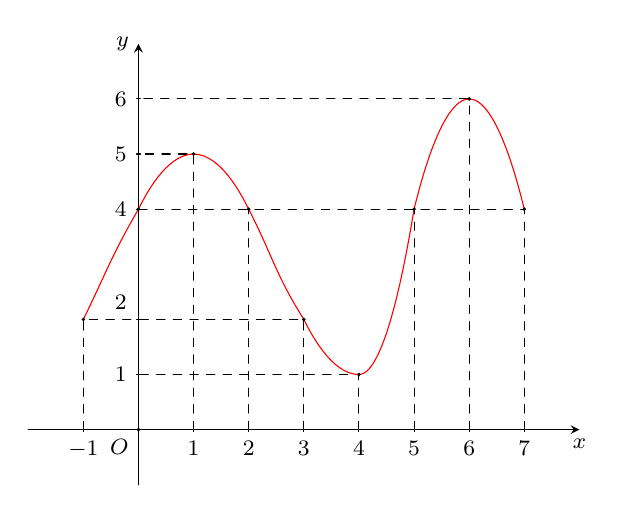
\begin{tikzpicture}[scale=0.7, font=\footnotesize, line join=round, line cap=round, >=stealth]
			\def\xmin{-2} \def\xmax{8}
			\def\ymin{-1} \def\ymax{7} 
			\draw[->] (\xmin,0)--(\xmax,0) node [below]{$x$};
			\draw[->] (0,\ymin)--(0,\ymax) node [left]{$y$};
			\fill (0,0)circle (1pt)node[below left]{$O$};
			\foreach \x/\g in {-1/below,1/below,2/below,3/below,4/below,5/below,6/below,7/below}  \draw[thin] (\x,1pt)--(\x,-1pt) node[\g]{$\x$};
			\foreach \y/\g in {1/left,2/above left,4/left,5/left,6/left} \draw[thin] (1pt,\y)--(-1pt,\y) node[\g]{$\y$};
			\draw[dashed] (-1,0)--(-1,2)--(0,2) (1,0)--(1,5)--(0,5) 
			(2,0)--(2,4)
			(3,0)--(3,2)--(0,2)
			(4,0)--(4,1)--(0,1)
			(5,0)--(5,4)
			(6,0)--(6,6)--(0,6)
			(7,0)--(7,4)--(0,4)
			;
			\draw[red] (0,4) parabola bend (1,5) (2,4) (3,2) parabola bend (4,1) (5,4)
			(5,4) parabola bend (6,6) (7,4) 
			;
			\draw[red] (-1,2)..controls+(64:1) and+(240:1)..(0,4)
			(2,4)..controls+(297:1) and+(122:1)..(3,2)
			;
			\fill (-1,2)circle(1pt)
			(0,4)circle(1pt)
			(1,5)circle(1pt)
			(2,4)circle(1pt)
			(3,2)circle(1pt)
			(4,1)circle(1pt)
			(5,4)circle(1pt)
			(6,6)circle(1pt)
			(7,4)circle(1pt)
			;
		\end{tikzpicture}
	\end{center}
	\loigiai{
		Hàm số $y=f(x)$ có:
		\begin{itemize}
			\item $x=1$ là điểm cực đại vì $f(x)<f(1)$ với mọi $x \in(0;2) \setminus\{1\}$,  $y_{\text{CĐ}}=f(1)=5$;
			\item $x=6$ là điểm cực đại vì $f(x)<f(6)$ với mọi $x \in(5;7) \setminus\{6\}$,  $y_{\text{CĐ}}=f(6)=6$;
			\item $x=4$ là điểm cực tiểu vì $f(x)>f(4)$ với mọi $x \in(3;5) \setminus\{4\}$, $y_{\text{CT}}=f(4)=1$.
		\end{itemize}
	}
\end{vd}

\begin{dang}{Tìm cực trị của hàm số bằng công thức}
	{\bf{Phương pháp giải}}
	\begin{itemize}
		\item \textit{Bước 1.} Tìm tập xác định $\mathscr{D}$ của hàm số.
		\item \textit{Bước 2.} Tính đạo hàm $f'(x)$. Tìm các điểm mà tại đó $f'(x)=0$ hoặc $f'(x)$ không xác định.
		\item \textit{Bước 3.} Xét dấu $f '(x)$ và xác định cực trị
		\begin{itemize}
			\item Lập bảng biến thiên.
			\item Dựa vào sự đổi dấu của $f'(x)$ khi $x$ đi qua các điểm tìm được ở Bước 2:
			\begin{itemize}
				\item Nếu $f '(x)$  đổi dấu từ dương sang âm khi $x$ đi qua $x_0$ thì $x_0$ là điểm cực đại. Giá trị cực đại là $f(x_0)$.
				\item Nếu $f '(x)$  đổi dấu từ âm sang dương khi $x$ đi qua $x_0$ thì $x_0$ là điểm cực tiểu. Giá trị cực tiểu là $f(x_0)$.
				\item Nếu $f '(x)$  không đổi dấu  khi $x$ đi qua $x_0$ thì $x_0$ không phải là điểm cực trị.
			\end{itemize}
		\end{itemize}
	\end{itemize}
\end{dang}
\begin{vd}%[TeX hóa SGK CTST 12]%[2D1H2-1]
	Tìm cực trị của hàm số $f(x)=2x^3-9x^2-24x+1$.
	\loigiai{
		Tập xác định $\mathscr{D}=\mathbb{R}$.\\
		Ta có $f'(x)=6x^2-18x-24$.\\
		Xét $f'(x)=0 \Leftrightarrow \hoac{&x=-1\\& x=4.}$\\
		Bảng biến thiên
		\begin{center}
			
\begin{tikzpicture}
				\tkzTabInit[nocadre=true,lgt=1.2,espcl=2.5,deltacl=0.6]
				{$x$ /0.6,$f'(x)$ /0.6,$f(x)$ /2}
				{$-\infty$,$-1$,$4$,$+\infty$}
				\tkzTabLine{,+,$0$,-,$0$,+,}
				\tkzTabVar{-/$-\infty$,+/$14$,-/$-111$,+/$+\infty$}
			\end{tikzpicture}
		\end{center}
		Vậy hàm số đạt cực đại tại $x=-1$, $y_{\text{CĐ}}=f(-1)=14$.\\
		Hàm số đạt cực tiểu tại $x=4$, $y_{\text{CT}}=f(4)=-111$.
	}
\end{vd}
\begin{vd}%[TeX hóa SGK CTST 12]%[Nguyễn Tiến]%[2D1H2-1]
	Tìm cực trị của hàm số $g(x)=\dfrac{x^2+x+4}{x+1}$.
	\loigiai{
		Tập xác định $\mathscr{D}=\mathbb{R}\setminus \{-1\}$.\\
		Ta có $g(x)=x+\dfrac{4}{x+1} \Rightarrow g'(x)=1-\dfrac{4}{(x+1)^2}=\dfrac{x^2+2x-3}{(x+1)^2}$;\\
		$g'(x)=0 \Leftrightarrow x^2+2x-3=0 \Leftrightarrow \hoac{& x=-3\\& x=1.}$\\
		Bảng biến thiên
		\begin{center}
			
\begin{tikzpicture}
				\tkzTabInit[nocadre=true,lgt=1.2,espcl=2.5,deltacl=0.6]
				{$x$ /0.6,$g'(x)$ /0.6,$g(x)$ /2}
				{$-\infty$,$-3$,$-1$,$1$,$+\infty$}
				\tkzTabLine{,+,$0$,-,d,-,$0$,+,}
				\tkzTabVar{-/$-\infty$,+/$-5$,-D+/$-\infty$/$+\infty$,-/$3$,+/$+\infty$}
			\end{tikzpicture}
		\end{center}
		Vậy hàm số đạt cực đại tại $x=-3$, $y_{\text{CĐ}}=g(-3)=-5$.\\
		Hàm số đạt cực tiểu tại $x=1$, $y_{\text{CT}}=g(1)=3$.
	}
\end{vd}

\begin{dang}{Ứng dụng tính đơn điệu và cực trị vào bài toán thực tế}
	{\bf{Phương pháp giải}}
	\begin{itemize}
		\item \textit{Bước 1.} Chuyển đổi bài toán thực tế sang bài toán hàm số.
		\begin{itemize}
			\item Xác định đại lượng cần khảo sát (ví dụ: độ cao $h$, lợi nhuận $P$, $\ldots$).
			\item Xây dựng hàm số biểu diễn đại lượng đó theo một biến số khác (ví dụ: thời gian $t$, khoảng cách $x$, $\ldots$).
			\item Xác định miền giá trị của biến số trong ngữ cảnh bài toán (ví dụ: $0<t<8$).
		\end{itemize}
			\item \textit{Bước 2.} Áp dụng phương pháp tìm tính đơn điệu và cực trị của hàm số.
		\begin{itemize}
			\item Tính đạo hàm của hàm số.
			\item Tìm các điểm mà đạo hàm bằng $0$ hoặc không xác định trong miền xác định đã cho.
			\item Lập bảng biến thiên để xác định các khoảng đồng biến, nghịch biến và các điểm cực trị.				
		\end{itemize}
			\item \textit{Bước 3.} Diễn giải kết quả vào ngữ cảnh bài toán thực tế.
		\begin{itemize}
			\item Các điểm cực đại tương ứng với giá trị lớn nhất của đại lượng cần khảo sát.
			\item Các điểm cực tiểu tương ứng với giá trị nhỏ nhất của đại lượng cần khảo sát.
			\item Các khoảng đồng biến/nghi.ch biến cho biết xu hướng tăng/gia?m của đại lượng.
		\end{itemize}
	\end{itemize}
\end{dang}
\begin{vd}%[2D1H1-5]
	[SGK 12-Cùng Khám Phá]
	Thể tích $V$ của $1$ kg nước (tính bằng $\text{cm}^3$) ở nhiệt độ $T$ (đơn vị: $^\circ$C) khi $T$ thay đổi từ $0^\circ$C đến $30^\circ$C được cho xấp xỉ bởi công thức:
	\[V=999{,}87-0{,}06426T+0{,}0085043T^2-0{,}0000769T^3.\]
	(Nguồn: James Stewart, J. (2015). Calculus.Cengage Learning 8th edition, p.284)\\ Tìm nhiệt độ $T_0 \in \left(0;30\right)$ để kể từ nhiệt độ $T_0$ trở lên thì thể tích $V$ tăng (làm tròn kết quả đến hàng đơn vị).
	\loigiai{Xét hàm số $f\left(T\right)=V=999{,}87-0{,}06426T+0{,}0085043T^2-0{,}0000769T^3$.\\ Hàm số xác định trên khoảng $\left(0;30\right)$.\\
		Ta có $f'\left(T\right)=2{,}307 \cdot 10^{-4}T^2+0{,}0170086T-0{,}06426$.\\
		$f'\left(T\right)=0\Leftrightarrow \hoac{&x\approx 4\\&x\approx 70}\Leftrightarrow x\approx4$.\\
		Khi đó, ta có bảng biến biên
		\begin{center}
			\begin{tikzpicture}
				\tkzTabInit[nocadre=true, lgt=1.5,espcl=3]
				{$T$ /.7, $f’(T)$ /.7, $f(T)$ /2}
				{$0$,$4$,$30$}
				\tkzTabLine{ ,-,z,+,}
				\path
				(N12)node[below](1){$f(0)$}
				(N23)node[above](2){$f(4)$}
				(N32)node[below](3){$f(30)$}
				;
				\foreach \x/\y in {1/2,2/3}
				\draw[-stealth] (\x)--(\y);
			\end{tikzpicture}
		\end{center}
		Vậy $T_0=4^\circ$C trở lên thì nhiệt độ tăng.
	}
\end{vd}

\begin{vd}%[2D1H2-1]
	[SGK CTST 12]
	Một phần lát cắt của dãy núi có độ cao tính bằng mét được mô tả bởi hàm số
	$$y=h(x)=-\dfrac{1}{1\,320\,000}x^3+\dfrac{9}{3\,520}x^2-\dfrac{81}{44}x+840, \text { với } 0\leq x\leq 2\,000.$$
	Tìm tọa độ các đỉnh của lát cắt dãy núi trên đoạn $[0; 2\,000]$.
	\begin{center}
		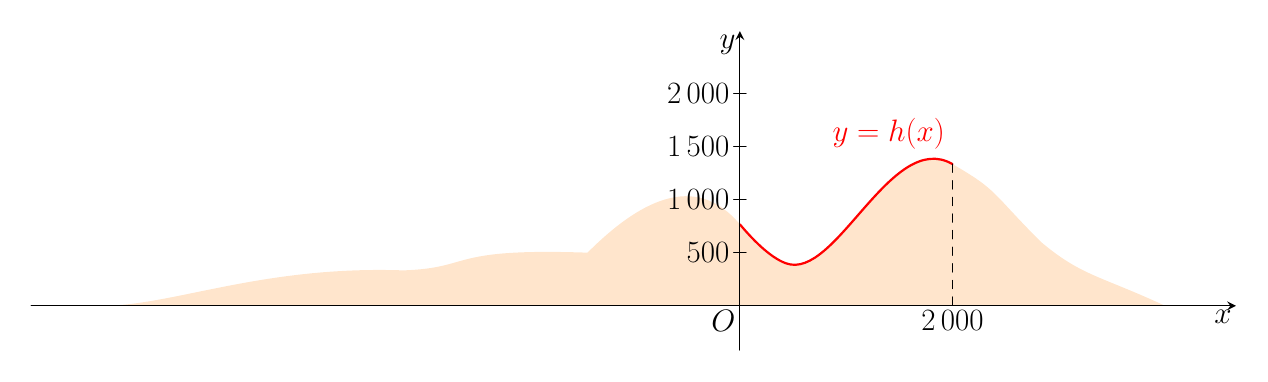
\begin{tikzpicture}[font=\footnotesize, line join=round, line cap=round, >=stealth,scale=0.45,transform shape]
			\def\xmin{-20} \def\xmax{14}
			\def\ymin{-1.25} \def\ymax{7.75}
			\clip (\xmin-.1,\ymin-.1) rectangle (\xmax+.1,\ymax+.1);
			
			\fill[orange!20] (-18,0)..controls+(0:2) and+(178:4) ..(-9.5,1)
			..controls+(2:2) and+(178:4) ..(-4.3,1.5)
			..controls+(45:2) and+(130:2) ..(0,2.3)
			..controls+(-50:.5) and+(160:.5) ..(1.3,1.2)
			..controls+(-20:1.5) and+(150:2) ..(6,4)
			..controls+(-30:1.5) and+(135:2) ..(8.5,1.8)
			..controls+(-40:1.5) and+(155:2) ..(12 ,0)--cycle
			;
			\draw[thick,red] (0,2.3)
			..controls+(-50:.5) and+(160:.5) ..(1.3,1.2)
			..controls+(-20:1.5) and+(150:2) ..(6,4);
			
			\draw[->] (\xmin,0)--(\xmax,0) node [below left]{\Huge $x$};
			\draw[->] (0,\ymin)--(0,\ymax) node [below left]{\Huge $y$};
			\node at (0,0) [below left]{\Huge $O$};
			\node at (4.2,4.3) [thick,red,above]{\Huge $y=h(x)$};
			\draw[dashed](6,4)--(6,0) node[below] {\Huge $2\,000$};
			\foreach \y/\diem in {1.5/500,3/1\,000,4.5/1\,500,6/2\,000}
			\draw[shift={(0,\y)},color=black] (5pt,0pt) -- (-5pt,0pt) node[left]{\Huge $\diem$};
		\end{tikzpicture}
	\end{center}
	\loigiai{
		Trên đoạn $[0; 2\,000]$, ta có $y'=-\dfrac{1}{440\,000}x^2+\dfrac{9}{1\,760}x^2-\dfrac{81}{44}$.\\
		Suy ra $y'=0 \Leftrightarrow \hoac{& x=450\\& x=1\,800.}$\\
		Bảng biến thiên
		\begin{center}
			
\begin{tikzpicture}
				\tkzTabInit[nocadre=true,lgt=1.2,espcl=3,deltacl=0.6]
				{$x$ /0.6,$y'$ /0.6,$y$ /2}
				{$0$,$450$,$1\,800$,$2000$}
				\tkzTabLine{,-,$0$,+,$0$,-,}
				\tkzTabVar{+/$840$,-/$\dfrac{7365}{16}$,+/$\dfrac{15\,315}{11}$,-/$\dfrac{43720}{33}$}
			\end{tikzpicture}
		\end{center}
		Vậy tọa độ các đỉnh là $\left(450; \dfrac{7365}{16}\right)$, và $\left(1\,800, \dfrac{15\,315}{11}\right)$.
	}
\end{vd}
\begin{vd}%[2D1H1-5]
	[SGK12-Cánh Diều]
	\immini{
		Máng trượt của một cầu trượt cho trẻ em (\textit{Hình a}) được uốn từ một tấm kim loại có bề rộng $80$ cm, mặt cắt được mô tả ở \textit{Hình b}. Nhà thiết kế khuyến cáo, diện tích mặt cắt càng lớn thì càng đảm bảo an toàn cho trẻ em.
		\begin{enumerate}
			\item Gọi $S$ là diện tích mặt cắt. Tìm điều kiện của $x$ và viết công thức tính $S$ theo $x$.
			\item Diện tích mặt cắt sẽ tăng hay giảm khi chúng ta tăng giá trị của $x$ từ 0 cm đến 10 cm?
		\end{enumerate}
	}{
		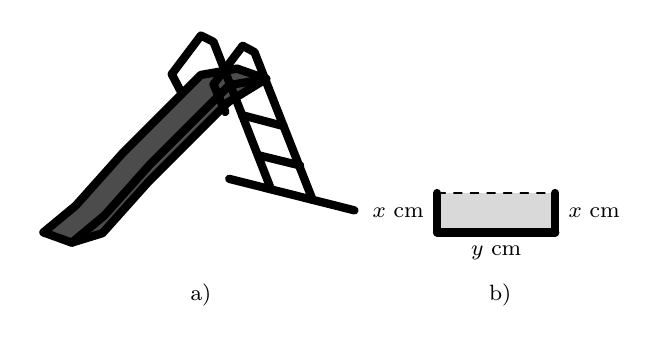
\begin{tikzpicture}[scale=1, font=\footnotesize, line join=round, line cap=round, >=stealth,line width=3.pt]
			\clip(-0.2,-1.2) rectangle (7.5,2.6);
			\fill[line width=3.pt,color=black,fill=black,fill opacity=0.7] (0,0)--(0.41,0.34)--(1,1)--(1.76,1.76)--(2,2)--(2.46,2.08)--(2.83,1.95)--(2.34,1.65)--(1.34,0.65)--(0.75,-0.01)--(0.36,-0.13)-- cycle;
			\draw (0,0)--(0.41,0.34)--(1,1)--(2,2)--(2.46,2.08);
			\draw (0,0)--(0.36,-0.13)--(0.77,0.21)--(0.77,0.21)--(1.36,0.87)--(2.36,1.87)--(2.83,1.95);
			\draw (0.36,-0.13)--(0.75,-0.01)--(1.34,0.65)--(2.34,1.65);
			\draw (2.36,0.68)-- (3.95,0.28);
			\draw (3.42,0.41)--(2.68,2.29)--(2.53,2.37)--(2.16,1.88)--(2.31,1.53);
			\draw (1.63,2.01)--(2,2.5)-- (2.16,2.42)--(2.89,0.55);
			\draw (1.63,2.01)--(1.76,1.76) (2.73,0.98)--(3.26,0.85) (2.52,1.49)--(3.05,1.35);
			\draw (2.34,1.65)--(2.83,1.95)--(2.46,2.08);
			\draw (2,-0.8)node{a)};
			\fill[line width=3.pt,fill=gray,fill opacity=0.3] (5,0.5)--(5,0)--(6.5,0)--(6.5,0.5)--cycle;
			\draw (5,0.5)--(5,0) node [left ,sloped,pos=0.5,rotate=90] {$x$ cm};
			\draw (5,0)--(6.5,0) node [below,sloped,pos=0.5] {$y$ cm};
			\draw (6.5,0)--(6.5,0.5) node [right,sloped,pos=0.5,rotate=-90] {$x$ cm};
			\draw[dashed,thin] (5,0.5)--(6.5,0.5);
			\draw (5.8,-0.8)node{b)};
			%			\draw (4,-1)node{\textit{Hình 5}};
		\end{tikzpicture}
	}
	\loigiai{
		\begin{enumerate}
			\item Do tấm kim loại có bề rộng $80 \mathrm{~cm}$ nên ta có $2x+y=80 \Leftrightarrow y=80-2x$.\\
			Để có thể thiết kế được máng trượt thì $y>0 \Leftrightarrow 80-2 x>0 \Leftrightarrow x<40$. Suy ra $0<x<40$.\\
			Diện tích của mặt cắt máng trượt là: $S=x y=x(80-2x)=-2x^2+80x$.		
			\item Ta có $S(x)=-2x^2+80x \text{ với } x\in(0; 40)$.
			\allowdisplaybreaks
			\begin{eqnarray*}
				S'(x)&=&-4 x+80 \\
				S'(x)&=&0 \Leftrightarrow-4 x+80=0 \Leftrightarrow x=20.
			\end{eqnarray*}
			Bảng biến thiên của hàm số $S(x)$ như sau
			\begin{center}
				
\begin{tikzpicture}
					\tkzTabInit[nocadre=true,lgt=1.2,espcl=2.5,deltacl=0.6,lw=.75pt]
					{$x$ /0.7, $S'(x)$ /0.7, $S(x)$ /2}
					{$0$,$20$,$40$}
					\tkzTabLine{ ,+,,-, }
					\tkzTabVar{-/$0$,+/$800$,-/$0$}
				\end{tikzpicture}
			\end{center}
			Vậy từ khi $x$ tăng từ $0$ cm đến $20$ cm thì diện tích mặt cắt sẽ tăng dần.
		\end{enumerate}
	}
\end{vd}

%-----------------------------------------------------------------------------
\subsection{Bài tập rèn luyện}
\ind{PHẦN I.} \inden{Câu trắc nghiệm nhiều phương án lựa chọn. Mỗi câu hỏi học sinh chỉ chọn một phương án.}\\
\setcounter{ex}{0}
\Opensolutionfile{ans}[ans/2D1-Bai1-TN]%--Đặt tên 2D1-Bai1-Dang1-TN
\begin{ex}%[2D1N1-2]
	[Trích đề thi khảo sát lần 2- Sở Nghệ An lần 2-Năm học 2024-2025]
	Cho hàm số $y=f(x)$ có bảng biến thiên như hình vẽ.
	\begin{center}
		\begin{tikzpicture}
			\tkzTabInit[nocadre=true, lgt=1, espcl=2.5, deltacl=0.5]
			{$x$/0.7, $y'$/0.7, $y$/2}
			{$-\infty$, $-1$, $0$, $1$, $+\infty$}
			\tkzTabLine{,+, 0,-, d,-, 0,+}
			\tkzTabVar{-/$-\infty$,+/$2$,-D+/$-\infty$/$+\infty$,-/$4$,+/$+\infty$}
			\node at (T11){\href{1G25OD}{\tiny \phantom{1G25OD}}};
		\end{tikzpicture}
	\end{center}
	Hàm số nghịch biến trên khoảng nào dưới đây?
	\choice
	{$(-\infty;-1)$}
	{$(4;+\infty)$}
	{$(-1;1)$}
	{\True $(0;1)$}
	\loigiai{
		Dựa vào bảng biến thiên, ta thấy hàm số nghịch biến trên khoảng $(0;1)$.
	}
\end{ex}
\begin{ex}%[2D1N2-2]
	[Trích đề thi khảo sát-Sở Hậu Giang-Năm học 2024-2025]
	Cho hàm số bậc ba $y=f(x)$ có bảng biến thiên như hình vẽ bên dưới
	\begin{center}
		
\begin{tikzpicture}[>=stealth]
			\tkzTabInit[nocadre=true,lgt=1,espcl=2.5,deltacl=0.5]{$x$/.7 ,$y'$/.7,$y$/2}
			{$-\infty$ , $1$ , $2$ , $+\infty$}
			\tkzTabLine{ ,+, $0$ ,-, $0$ ,+, }
			\tkzTabVar{-/$-\infty$ ,+/$0$ , -/$-1$ ,+/$+\infty$}
		\end{tikzpicture}
	\end{center}
	Hàm số đã cho đạt giá trị cực đại tại điểm
	\choice
	{$x=-1$}
	{$x=0$}
	{$x=2$}
	{\True $x=1$}
	\loigiai{
		Nhìn vào bảng biến thiên ta có hàm số đã cho đạt cực đại tại điểm $x=1$.}
\end{ex}
\begin{ex}%[2D1N2-2]
	[Trích đề thi khảo sát-Sở Bà Rịa Vũng Tàu-Năm học 2024-2025]
	Cho hàm số $y=f(x)$ có bảng biến thiên như sau
	\begin{center}
		
\begin{tikzpicture}[>=stealth]
			\tkzTabInit[nocadre=true,lgt=1,espcl=2,deltacl=0.5]{$x$/.7 ,$y'$/.7,$y$/2}
			{$-\infty$ , $-2$ , $0$ , $2$ , $+\infty$}
			\tkzTabLine{ ,-, $0$ ,+, $0$ ,-, $0$ ,+, }
			\tkzTabVar{+/$+\infty$ , -/$1$,+/$3$ , -/$1$ ,+/$+\infty$}
		\end{tikzpicture}
	\end{center}
	Giá trị cực đại của hàm số đã cho là
	\choice
	{$2$}
	{\True $3$}
	{$1$}
	{$0$}
	\loigiai{
		Quan sát bảng biến thiên ta thấy hàm số đạt cực đại tại điểm $x=0$ và giá trị cực đại của hàm số là $y_{\text{CĐ}}=3$.
	}
\end{ex}
\begin{ex}%[2D1N1-2]
	[Trích đề thi khảo sát-Sở Hải Dương-Năm học 2024-2025]
	Cho hàm số $y=f(x)$ có bảng biến thiên như sau
	\begin{center}
		
\begin{tikzpicture}[>=stealth]
			\tkzTabInit[nocadre=true,lgt=1.5,espcl=2.5,deltacl=0.6]{$x$/.7 ,$f'(x)$/.7,$f(x)$/2}
			{$-\infty$ , $-1$ , $0$ , $+\infty$}
			\tkzTabLine{ ,-, $0$ ,+, $0$ ,-, }
			\tkzTabVar{+/$+\infty$ , -/$0$ ,+/$2$ , -/$-\infty$}
		\end{tikzpicture}
	\end{center}
	Khẳng định nào dưới đây là đúng?
	\choice
	{Hàm số nghịch biến trên khoảng $(-1;+\infty)$}
	{\True Hàm số đồng biến trên khoảng $(-1;0)$}
	{Hàm số nghịch biến trên khoảng $(-\infty;0)$}
	{Hàm số đồng biến trên khoảng $(0;2)$}
	\loigiai{
		Từ bảng biến thiên ta thấy, hàm số đã cho đồng biến trên khoảng $(-1;0)$.
	}
\end{ex}
\begin{ex}%[2D1N1-2]
	[Trích đề thi khảo sát-Sở Hưng Yên-Năm học 2024-2025]
	Cho hàm số $y=f(x)$ có bảng biến thiên như hình vẽ bên dưới.
	\begin{center}
		
\begin{tikzpicture}
			\tkzTabInit[nocadre=true,lgt=1.2,espcl=2.5,deltacl=0.6]
			{$x$/0.6,$f'(x) $/0.6,$f(x)$/2}
			{$-\infty$,$-2$,$3$,$+\infty$}
			\tkzTabLine{,+,0,-,0,+,} %
			\tkzTabVar{-/$-\infty$,+/$4$, -/$2$,+/$+\infty$} %dấu mũi tên,+trên, -dưới
		\end{tikzpicture}
	\end{center}
	Hàm số $y=f(x)$ đồng biến trên khoảng nào dưới đây?
	\choice
	{$(-1;2)$}
	{\True $(-8;-3)$}
	{$(-\infty; 4)$}
	{$(2;+\infty)$}
	\loigiai{
		Từ bảng biến thiên ta thấy hàm số đồng biến trên các khoảng $(-\infty;-2)$ và $(3;+\infty)$.\\
		Mà $(-8;-3) \subset(-\infty;-2)$ nên suy ra hàm số $y=f(x)$ đồng biến trên khoảng $(-8;-3)$.
	}
\end{ex}
\begin{ex}%[2D1N1-2]
	[Trích đề thi khảo sát-Sở Thừa Thiên Huế-Năm học 2024-2025]
	Cho hàm số $y=f(x)$ có bảng biến thiên như sau:
	\begin{center}
		\resizebox{0.7\linewidth}{!}{
\begin{tikzpicture}[font=\normalsize,t style/.style={style=solid}]
				\tkzTabInit[nocadre=true, lgt=1.4, espcl=3, deltacl=0.65]
				{$x$/0.75, $f'(x)$/0.75, $f(x)$/2.5}
				{$-\infty$, $-3$, $0$, $3$, $+\infty$}
				\tkzTabLine{ , -, 0,+, 0, -, 0,+}
				\tkzTabVar{+/$+\infty$, -/$-1$,+/$1$, -/$-1$,+/$+\infty$}
		\end{tikzpicture}}
	\end{center}
	Hàm số đã cho đồng biến trên khoảng nào dưới đây?
	\choice
	{$(-\infty;-3)$}
	{$(-3;3)$}
	{$(0;3)$}
	{\True $(-3;0)$}
	\loigiai{
		Hàm số đã cho đồng biến trên khoảng $\left( -3;0 \right)$ và $\left( 3\,;\,+\infty  \right)$.
	}
\end{ex}
\begin{ex}%[2D1N2-2]
	[Trích đề thi thử Chuyên KHTN-Hà Nội- Lần 2-Năm học 2024-2025]
	Cho hàm số $y=f(x)$ có bảng biến thiên như sau
	\begin{center}
		
\begin{tikzpicture}
			\tkzTabInit[nocadre=true,lgt=1.5,espcl=2.5,deltacl=0.6]
			{$x$/0.7,$f'(x)$/0.7,$f(x)$/1.5}
			{$-\infty$,$-2$,$1$,$+\infty$}
			\tkzTabLine{,+,0,-,0,+,}
			\tkzTabVar{-/$-\infty$,+/$21$,-/$-6$,+/$+\infty$}
		\end{tikzpicture}
	\end{center}
	Điểm cực đại của hàm số đã cho là
	\choice
	{$21$}
	{$1$}
	{\True $-2$}
	{$-6$}
	\loigiai{
		Từ bảng biến thiên suy ra điểm cực đại của hàm số đã cho là $x=-2$.
	}
\end{ex}
\begin{ex}%[2D1N1-2]
	[Trích đề thi HK1-Lớp 12-THPT Lương Ngọc Quyến-Thái Nguyên-Năm học 2024-2025]
	Cho hàm số $y=f(x)$ có bảng biến thiên như hình dưới đây
	\begin{center}
		
\begin{tikzpicture}
			\tkzTabInit[nocadre=true,lgt=1,espcl=2.1]
			{$x$ /0.6,$y'$ /0.6,$y$ /2}
			{$-\infty$,$-7$,$-4$,$4$,$+\infty$}
			\tkzTabLine{,-,$0$,+,d,+,$0$,-,}
			\tkzTabVar{+/$+\infty$, -/$14$,+D-/$+\infty$/$-\infty$,+/$6$,-/$-\infty$}
		\end{tikzpicture}
	\end{center}
	Hàm số đồng biến trên khoảng nào trong các khoảng sau đây?
	\choice
	{$(-7;4)$}
	{$(-7;+\infty)$}
	{$(-\infty;-4)$}
	{\True $(-7;-4)$ và $(-4;4)$}
	\loigiai{
		Dựa vào bảng biến thiên ta có hàm số đồng biến trên khoảng $(-7;-4)$ và $(-4;4)$.
	}
\end{ex}
\begin{ex}%[2D1N1-1]
	[Trích đề thi HK1-Lớp 12 -Sở GDĐT Bắc Giang-Năm học 2024-2025]
	Hàm số nào dưới đây đồng biến trên $\mathbb{R}$?
	\choice 
	{$y=x^2+2x+3$}
	{\True $y=x^3+x+1$}
	{$y=-x^3-3x$}
	{$y=\dfrac{x+1}{x+3}$} 
	\loigiai{
		Xét hàm số $y=x^3+x+1$ có $y'=3x^2+1 \ge 0,\forall x \in \mathbb{R}$.\\
		Do đó hàm số đã cho đồng biến trên $\mathbb{R}$.}
\end{ex}
\begin{ex}%[2D1H1-2]
	[Trích đề thi HK1-Lớp 12 -THPT Nguyễn Thái Bình-TPHCM-Năm học 2024-2025]
	Cho hàm số $y=f(x)$ có bảng biến thiên
	\begin{center}
		
\begin{tikzpicture}
			\tkzTabInit[espcl=2.5,lgt=1.5,nocadre]
			{$x$/0.7,$y'$/0.7,$y$/2.1}
			{$-\infty$,$-1$,$1$,$+\infty$}
			\tkzTabLine{,-,0,+,0,-,}
			\tkzTabVar{+/$+\infty$,-/$0$,+/$4$,-/$-\infty$}
		\end{tikzpicture}
	\end{center}
	Chọn khẳng định đúng?
	\choice
	{\True Hàm số đồng biến trên $(-1; 1)$}
	{Hàm số đồng biến trên $(-\infty;-1)$}
	{Hàm số nghịch biến trên $(-1; 1)$}
	{Hàm số nghịch biến trên $(-1;+\infty)$}
	\loigiai{
		Dựa vào bảng biến thiên, ta thấy hàm số đồng biến trên $(-1; 1)$.
	}
\end{ex}
\begin{ex}%[2D1N2-2]
	[Trích đề thi HK1-Lớp 12 -THPT Chu Văn An-Quãng-Nam-Năm học 2024-2025]
	Hàm số $y=f(x)$ xác định, liên tục trên $\mathbb{R}$ và có bảng biến thiên như hình vẽ bên dưới. Khẳng định nào sau đây đúng?
	\begin{center}
		
\begin{tikzpicture}
			\tkzTabInit[nocadre=true,lgt=1.2,espcl=2.5,deltacl=0.6]
			{$x$ /0.6,$y'$ /0.6,$y$ /2}
			{$-\infty$,$0$,$1$,$2$,$+\infty$}
			\tkzTabLine{,+,d,+,0,-,$0$,+,}
			\tkzTabVar{-/$-\infty$,R/,+/$1$,-/$-1$,+/$0$}
			\tkzTabIma{1}{5}{2}{$0$} 			
		\end{tikzpicture}
	\end{center}
	\choice
	{\True Hàm số có đúng hai cực trị}
	{Hàm số đạt cực tiểu tại $x=-1$}
	{Hàm số có giá trị lớn nhất bằng $1$ và giá trị nhỏ nhất bằng $-1$}
	{Hàm số đạt cực đại tại $x=0$, $x=1$ và đạt cực tiểu tại $x=2$}
	\loigiai{
		Theo bảng biến thiên $y'$ đổi dấu qua $x=1$, $x=2$ nên hàm số có đúng hai cực trị.
	}
\end{ex}
\begin{ex}%[2D1H1-1]
	[Trích đề thi HK1-Lớp 12-THPT Đinh Tiên Hoàng-Tỉnh Ninh Bình-Năm học 2024-2025]
	Cho hàm số $=f(x)$ có đạo hàm $f'(x)=x^2-4x$, $\forall x\in \mathbb{R}$. Khẳng định nào sau đây đúng?	
	\choice
	{$f(4)>f(0)$}
	{$f(5)>f(6)$}
	{\True $f(0)>f(2)$}
	{$f(4)>f(2)$}
	\loigiai{
		Ta có $f'(x)=0\Leftrightarrow x^2-4x=0\Leftrightarrow \hoac{&x=0\\&x=4.}$\\
		Từ đó ta có bảng biến thiên sau
		\begin{center}
			
\begin{tikzpicture}
				\tkzTabInit[nocadre=true,lgt=1.2,espcl=2.5,deltacl=0.6]
				{$x$ /0.6, $f'(x)$ /0.6}
				{$-\infty$,$0$,$4$,$+\infty$}
				\tkzTabLine{,+,$0$,-,$0$,+,}
			\end{tikzpicture}
		\end{center}
		Vì hàm số nghịch biến trong $(0;4)$ nên $f(0)>f(2)$.	
	}
\end{ex}
\begin{ex}%[2D1H2-3]
	[Lớp 12-Đề thi HK1- NH24-25-TH-THCS-THPT Lê Thánh Tông-TPHCM]
	Với giá trị nào của $m$ thì hàm số $y=\dfrac{1}{3} x^3-m x^2+\left(m^2-m-1\right) x$ đạt cực đại tại $x=1$?
	\choice
	{$m=1$}
	{$m=2$}
	{\True $m=3$}
	{$m=4$}
	\loigiai{Ta có $y'=x^2-2mx+m^2-m-1$.
		\\
		Để  hàm số $y=\dfrac{1}{3} x^3-m x^2+\left(m^2-m-1\right) x$ đạt cực đại tại $x=1$ thì 
		\[y'(1)=0\Leftrightarrow 1-2m+m^2-m-1=0\Leftrightarrow m^2-3m=0\Leftrightarrow\hoac{&m=0\\&m=3.}\]
		\begin{itemize}
			\item Với $m=0$, $y'=x^2-1=0\Leftrightarrow \hoac{&x=1\\&x=-1.}$\\
			Ta có bảng biến thiên như sau
			\begin{center}
				
\begin{tikzpicture}[>=stealth,scale=0.8,line cap=round,line join=round]
					\tkzTabInit[lgt=1.2,espcl=2.5,deltacl=0.6]
					{$x$/1,$y'$/1,$y$/3}
					{$-\infty$,$-1$,$1$,$+\infty$}
					\tkzTabLine{,+,0,-,0,+,} %
					\tkzTabVar{-/$-\infty$,+/, -/,+/$+\infty$} %dấu mũi tên,+trên, -dưới
				\end{tikzpicture}
			\end{center}
			Suy ra với $m=0$ không thỏa mãn bài toán.
			\item  Với $m=3$, $y'=x^2-6x+5=0\Leftrightarrow \hoac{&x=1\\&x=5.}$\\
			Ta có bảng biến thiên như sau
			\begin{center}
				
\begin{tikzpicture}[>=stealth,scale=0.8,line cap=round,line join=round]
					\tkzTabInit[lgt=1.2,espcl=2.5,deltacl=0.6]
					{$x$/1,$y'$/1,$y$/3}
					{$-\infty$,$1$,$5$,$+\infty$}
					\tkzTabLine{,+,0,-,0,+,} %
					\tkzTabVar{-/$-\infty$,+/, -/,+/$+\infty$} %dấu mũi tên,+trên, -dưới
				\end{tikzpicture}
			\end{center}
			Suy ra với $m=3$  thỏa mãn bài toán.
		\end{itemize}
		
	}
\end{ex}

\begin{ex}%[2D1H1-1]
	[Trích đề thi HK1-Lớp 12 -PT DTNT-Tỉnh Phú Yên-Năm học 2024-2025]
	Hàm số $y=\dfrac{2x+8}{5x-9}$ nghịch biến trên khoảng nào trong các khoảng sau?
	\choice
	{$(0 ;+\infty)$}
	{$(-\infty ;+\infty)$}
	{\True $(2 ;+\infty)$}
	{$(-\infty ; 5)$}
	\loigiai{Hàm số $y=\dfrac{2x+8}{5x-9}$ nghịch biến trên các khoảng $\left(-\infty;\dfrac{9}{5}\right)$ và $\left(\dfrac{9}{5};+\infty\right)$.}
\end{ex}
%%%==============HetCau_EX20==============%%%
\begin{ex}%[2D1H2-1]
	[Trích đề thi HK1-Lớp 12 -THPT Tam Phu-Tp HCM-Năm học 2024-2025]
	Hàm số nào dưới đây \textbf{không} có cực trị?
	\choice
	{$y=x^2-2x+1$}
	{$y=\dfrac{x^2+1}{x}$}
	{$y=-x^3+x+1$}
	{\True $y=\dfrac{2x-2}{x+1}$}
	\loigiai{
		Do $y'=\left(\dfrac{2x-2}{x+1}\right)'=\dfrac{4}{(x+1)^2}>0$, $\forall x\ne -1$ nên hàm số này không có cực trị.
	}
\end{ex}
\begin{ex}%[2D1H2-1]
	[Trích đề thi HK1-Lớp 12 -THPT Lê Trọng Tấn-TPHCM-Năm học 2024-2025]
	Cho hàm số $f(x)$ có đạo hàm là $f'(x)=x(x-1)(x+2)^2$, $\forall x \in \mathbb{R}$. Số điểm cực trị của hàm số là?
	\choice
	{$5$}
	{\True $2$}
	{$1$}
	{$3$}
	\loigiai{
		Cho $f'(x)=0\Leftrightarrow \hoac{&x=0\\&x=1\\&x=-2\quad \text{(bội chẵn).}}$\\
		Suy ra hàm số $f(x)$ có $2$ điểm cực trị.
	}
\end{ex}


\begin{ex}%[2D1H2-2]
	[Trích đề thi HK1-Lớp 12 -THPT Nguyễn Thái Bình-TPHCM-Năm học 2024-2025]
	\immini{
		Cho hàm số $y=f(x)$ có đồ thị như hình vẽ. Điểm cực đại của đồ thị hàm số đã cho có tọa độ là
		\choice
		{\True $(1; 2)$}
		{$(-1; 2)$}
		{$(1;-2)$}
		{$(-1;-2)$}
	}
	{
		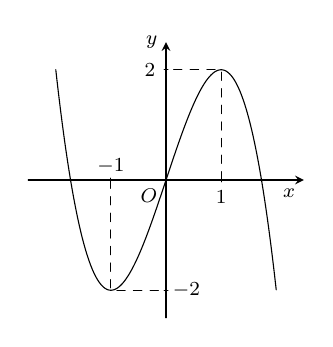
\begin{tikzpicture}[scale=.7, font=\footnotesize, line join=round, line cap=round, >=stealth]
			\tikzset{every node/.style={scale=0.9}}
			\draw[->] (-2.5,0)--(2.5,0) node[below left] {$x$};
			\draw[->] (0,-2.5)--(0,2.5) node[left] {$y$};
			\draw (0,0) node [below left] {$O$};
			\foreach \x/\nx in {1/1}
			\draw[thin] (\x,1pt)--(\x,-1pt) node [below] {$\nx$};
			\foreach \x/\nx in {-1/-1}
			\draw[thin] (\x,1pt)--(\x,-1pt) node [above] {$\nx$};
			\foreach \y/\ny in {2/2}
			\draw[thin] (1pt,\y)--(-1pt,\y) node [left] {$\ny$};
			\foreach \y/\ny in {-2/-2}
			\draw[thin] (1pt,\y)--(-1pt,\y) node [right] {$\ny$};
			\draw[dashed,thin](-1,0)--(-1,-2)--(0,-2);
			\draw[dashed,thin](1,0)--(1,2)--(0,2);
			\begin{scope}
				\clip (-2.5,-2.5) rectangle (2.5,2.5);
				\draw[samples=200,domain=-2:2,smooth,variable=\x] plot (\x,{-1*((\x)^3)+0*((\x)^2)+3*(\x)+0});
			\end{scope}
		\end{tikzpicture}		
	}
	\loigiai{
		Điểm cực đại của đồ thị hàm số đã cho có tọa độ $(1;2)$.
	}
\end{ex}
\begin{ex}%[2D1H5-5]
	[Trích đề thi HK1-Lớp 12 -THPT Đinh Tiên Hoàng-Tỉnh Ninh Bình-Năm học 2024-2025]
	\immini{Cho hàm số $y=f(x)$, có đồ thị hàm số $y=f'(x)$ như hình bên. Tìm số điểm cực trị của hàm số $y=f(x)$.	
		\choice
		{$3$}
		{\True $1$}
		{$0$}
		{$2$}}
	{\begin{tikzpicture}[scale=1,>=stealth, font=\footnotesize, line join=round, line cap=round]
			\def\xmin{-1} \def\xmax{5}
			\def\ymin{-1} \def\ymax{3}
			
			%	\draw[color=gray!50,dashed] (\xmin,\ymin) grid (\xmax,\ymax);
			
			\draw[->] (\xmin,0)--(\xmax,0) node [below]{$x$};
			\draw[->] (0,\ymin)--(0,\ymax) node [left]{$y$};
			\node at (0,0) [below left]{$O$};
			\draw plot[smooth,tension=0.7]coordinates {(-0.5,3) (1,0.5) (3,2) (4,-1)};
			\draw[fill=black]
			(0,0) circle (0.05);
	\end{tikzpicture}}
	\loigiai{
		Dựa vào đồ thị $f'(x)$ ta thấy đồ thị cắt $Ox$ tại duy nhất một điểm hay phương trình $f'(x)=0$ có $1$ nghiệm đơn. Từ đó ta có bảng biến thiên
		\begin{center}
			
\begin{tikzpicture}
				\tkzTabInit[nocadre=true,lgt=1.2,espcl=2.5,deltacl=0.6]
				{$x$ /0.6, $f'(x)$ /0.6}
				{$-\infty$,$x_1$,$+\infty$}
				\tkzTabLine{,+,$0$,-,}
			\end{tikzpicture}
		\end{center}
		Vậy hàm số $y=f(x)$ có một điểm cực trị.	
	}
\end{ex}

\begin{ex}%[2D1H1-3]
	[Trích đề thi GHK1-Lớp 12 -THPT Tam Phu-TP HCM-Năm học 2024-2025]
	Có tất cả bao nhiêu số nguyên $m$ để hàm số $y=\dfrac{(m+1) x-2}{x-m}$ đồng biến trên từng khoảng xác định của nó?
	\choice
	{$1$}
	{$3$}
	{$0$}
	{\True $2$}
	\loigiai{
		Tập xác định $\mathscr{D}=\mathbb{R} \setminus \left\{ m\right\} $.\\
		Ta có $ y'=\dfrac{-m^2-m+2}{(x-m)^2} $.\\
		Hàm số đồng biến trên từng khoảng xác định $\Leftrightarrow y'>0,\forall x\in\mathscr{D}\Leftrightarrow -m^2-m+2>0\Leftrightarrow -2<m<1 $.\\
		Các giá trị nguyên của $ m $ thỏa mãn là $ \{-1;0\} $.\\
		Vậy có hai giá trị nguyên  của $m$ thỏa mãn yêu cầu bài toán.
	}
\end{ex}

	\begin{ex}%[2D1H2-1]
		[Trích đề thi khảo sát-Lớp 12 -Sở Hải Phòng-Năm học 2024-2025]
	Cho hàm số nào $y=f(x)$ là hàm đa thức có đạo hàm $f'(x)=x\left( x^2-1 \right)\left( x-2 \right)^2$. Số điểm cực tiểu của đồ thị hàm số là
	\choice
	{$4$}
	{$1$}
	{\True $2$}
	{$3$}
	\loigiai{
		Ta có $f'(x)=x\left( x^2-1 \right)\left( x-2 \right)^2=0\Leftrightarrow \hoac{& x=0 \\ 	& x=-1 \\ 	& x=1 \\ & x=2 ~(\text{nghiệm kép}).}$ \\
		Bảng biến thiên
	\begin{center}
			
\begin{tikzpicture}
			\tkzTabInit[nocadre=true,lgt=1.2,espcl=2.5,deltacl=0.6]
			{$x$/0.7,$f'(x)$/0.7,$f(x)$/2}{$-\infty$,$-1$,$0$,$1$,$2$,$+\infty$}
			\tkzTabLine{,-,0,+,0,-,0,+,0,+,}   
			\tkzTabVar{+/,-/,+/,-/,R,+/ }
		\end{tikzpicture}
	\end{center}
		Dựa vào BBT ta thấy đồ thị hàm số có $2$ điểm cực tiểu.}
\end{ex}



\Closesolutionfile{ans}

\ind{PHẦN II.} \inden{Câu trắc nghiệm đúng sai. Trong mỗi ý a), b), c), d) ở mỗi câu, học sinh chọn đúng hoặc sai.}\\
\setcounter{ex}{0}
\Opensolutionfile{ans}[ans/2D1-Bai1-DS]%--Đặt tên 2D1-Bai1-DS
\begin{ex}%[2D1H2-1]
	[Trích đề thi GHKI-lớp 12-THPT Phan Chu Trinh- Bình Thuận-Năm học-2024-2025]
	Cho hàm số $f(x)=x^3-3x^2+3$. 
	\choiceTF
	{\True Hàm số nghịch biến trên khoảng $\left(0;2\right)$}
	{\True $f\left(10^6\right)<f\left(10^8\right)$}
	{Hàm số đạt cực đại tại $x=2$}
	{\True Tổng giá trị cực đại và giá trị cực tiểu của hàm số bằng $2$}
	\loigiai{
		Tập xác định $ \mathscr{D}=\mathbb{R} $.\\
		Ta có $ y'=3x^2-6x $.\\
		Xét $ y'=0\Leftrightarrow 3x^2-6x\Leftrightarrow\hoac{& x=0 \\ & x=2.} $\\
		Bảng biến thiên
		\begin{center}
			% Cần khai báo \usepackage{tkz-tab}
			
\begin{tikzpicture}[>=stealth]
				\tkzTabInit[nocadre=true,lgt=1,espcl=2.5,deltacl=0.5]{$x$/.7 ,$y'$/.7,$y$/2}
				{$-\infty$ , $0$ , $2$ , $+\infty$}
				\tkzTabLine{ ,+, $0$ ,-, $0$ ,+, }
				\tkzTabVar{-/$-\infty$ ,+/$3$ , -/$-1$ ,+/$+\infty$}
			\end{tikzpicture}
			
		\end{center}
		\begin{itemchoice}
			\itemch 
			Hàm số nghịch biến trên khoảng $ (0;2) $.
			\itemch 
			Hàm số đồng biến trên $ (2;+\infty) $ nên $f\left(10^6\right)<f\left(10^8\right)$.
			\itemch 
			Hàm số đạt cực đại tại $ x=0 $.
			\itemch  Ta có $ \heva{& M=y_{\text{CĐ}}=
				3 \\ &m=y_{\text{CT}} =-1 }\Rightarrow M+m=2 $.
		\end{itemchoice}
	}
\end{ex}
\begin{ex}%[2D1H5-8]
	[Trích đề thi khảo sát lần 1-Lớp 12 -SỞ LÀO CAI-Năm học 2024-2025]
	Khi loại thuốc A được tiêm vào bệnh nhân, nồng độ $(\mathrm{mg} / \mathrm{l})$ của thuốc trong máu sau $x$ phút (kể từ khi bắt đầu tiêm) được xác định bởi công thức $C(x)=\dfrac{30 x}{x^2+2}$.\\
	\textit{(Nguồn: James Stewart, J. (2015). Calculus. Cengage Learning)}
	\choiceTF
	{\True Thời điểm $1$ phút sau khi tiêm, nồng độ thuốc trong máu là $10(\mathrm{mg} / \mathrm{l})$}
	{\True  Đạo hàm của hàm số $C(x)$ là $C'(x)=\dfrac{-30x^2+60}{\left(x^2+2\right)^2}$}
	{Trong khoảng thời gian từ $1$ phút sau khi tiêm trở đi, nồng độ thuốc trong máu giảm dần}
	{Nồng độ thuốc trong máu đạt giá trị lớn nhất tại thời điểm $2$ phút sau khi tiêm}
	\loigiai{
		\begin{itemchoice}
			\itemch 	Ta có công thức xác định nồng độ $(\mathrm{mg} / \mathrm{l})$ của thuốc trong máu sau $x$ phút là $$C(x)=\dfrac{30 x}{x^2+2}.$$
			Với thời gian $1$ phút sau khi tiêm, ta thay $x=1$ vào $C(x)$, có
			$$
			C(1)=\dfrac{30}{3}=10(\mathrm{mg} / \mathrm{l}).
			$$	
			\itemch 	Ta có $C(x)=\dfrac{30 x}{x^2+2}$, suy ra
			\begin{eqnarray*}
				& 	C'(x)& =\dfrac{(30 x)'\cdot \left(x^2+2\right)-\left(x^2+2\right)'\cdot (30 x)}{\left(x^2+2\right)^2}\\
				& & 	=\dfrac{30\left(x^2+2\right)-2 x\cdot (30 x)}{\left(x^2+2\right)^2}\\
				& & 	=\dfrac{30 x^2+60-60 x^2}{\left(x^2+2\right)^2}\\
				& & =\dfrac{-30 x^2+60}{\left(x^2+2\right)^2}.
			\end{eqnarray*}
			
			\itemch 
			Cho $C'(x)=0$ hay $\dfrac{-30x^2+60}{\left(x^2+2\right)^2}=0 \Rightarrow -30x^2+60=0 \Leftrightarrow\hoac{&x=\sqrt{2} \\ &x=-\sqrt{2}.}$\\
			Ta có bảng biến thiên
			\begin{center}
				
\begin{tikzpicture}
					\tkzTabInit[nocadre,lgt=1.5,espcl=3,deltacl=.5]
					{$x$/0.7, $C’(x)$/0.7, $C(x)$/2}
					{$-\infty$,$-\sqrt{2}$,$\sqrt{2}$,$+\infty$}
					\tkzTabLine{,-,z,+,z,-,}
					\tkzTabVar{+/$+\infty$ ,-/ $-\dfrac{15\sqrt{2}}{2}$ ,+/$\dfrac{15\sqrt{2}}{2}$, -/$-\infty$}
				\end{tikzpicture}
			\end{center}
			Vậy khoảng thời gian từ $1$ phút sau khi tiêm trở đi, nồng độ thuốc tăng trên khoảng $\left(1 ; \sqrt{2}\right)$ và giảm trên khoảng $\left(\sqrt{2} ;+\infty\right)$.
			\itemch Nồng độ thuốc đạt giá trị lớn nhất sau $x=\sqrt{2} \approx 1{,}4$ phút.
		\end{itemchoice}
	}
\end{ex}
\begin{ex}%[2D1V1-2]
	[Trích đề thi GKI -Lớp 12 -THPT Lê Thánh Tông- Tp HCM-Năm học 2024-2025]
	\immini[thm]{Hàm số $y=f(x)$ xác định và liên tục trên $\mathbb{R}$. Hàm số $f'(x)$ có đồ thị như sau.
		\choiceTF
		{\True Hàm số $y=f(x)$ đồng biến trên khoảng $(0;2)$}
		{Hàm số $y=f(x)$ có hai điểm cực trị}
		{\True Hàm số $h(x)=f(x)+m$ nghịch biến trên khoảng $(-\infty;-1)$}
		{\True Hàm số $g(x)=f(1-2x)$ đồng biến trên khoảng $(1;+\infty)$}
	}
	{
		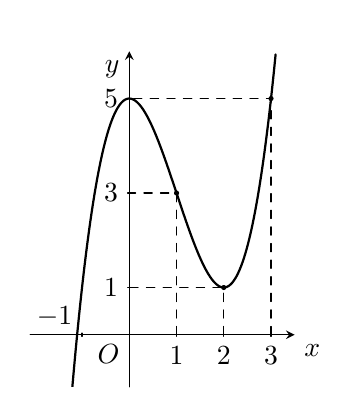
\begin{tikzpicture}[line join=round, line cap=round,>=stealth,scale=0.6]
			\draw[->] (-2.1,0)--(3.5,0) node[below right] {$x$};
			\draw[->] (0,-1.1)--(0,6) node[below left] {$y$};
			\draw (0,0) node [below left] {$O$};
			\draw[dashed,thin]
			(1,0)--(1,3)--(0,3)
			(2,0)--(2,1)--(0,1)
			(3,0)--(3,5)--(0,5)
			;
			\foreach \i/\j in {1/3,2/1,3/5}{
				\draw[fill=black] (\i,\j) circle (1.2pt);}
			\draw[thin] (-1,1pt)--(-1,-1pt) node [above left] {$-1$};
			\foreach \i in {1,2,3}
			{\draw[thin] (\i,1pt)--(\i,-1pt) node [below] {$\i$};}
			\foreach \j in {1,3,5}{\draw[thin] (1pt,\j)--(-1pt,\j) node [left] {$\j$};}
			\begin{scope}
				\clip (-2.1,-1.1) rectangle (3.5,6.5);
				\draw[thick,samples=200,domain=-3:3.1,smooth,variable=\x] plot (\x,{1*((\x)^3)-3*((\x)^2)+0*(\x)+5});
			\end{scope}
		\end{tikzpicture}
	}
	\loigiai{
		Từ đồ thị ta có $f'(x)=0\Leftrightarrow x=-1$.\\
		Ta có bảng biến thiên của $f(x)$ như sau
		\begin{center}
			
\begin{tikzpicture}
				\tkzTabInit[nocadre=true,lgt=1.2,espcl=3,deltacl=0.6]
				{$x$/1,$f'(x)$/1,$f(x)$/2}
				{$-\infty$,$-1$,$+\infty$}
				\tkzTabLine{,-,0,+,}   
				\tkzTabVar{+/$+\infty$,-/$ $,+/$+\infty$}
			\end{tikzpicture}
		\end{center}	
		Từ bảng biến thiên ta thấy hàm số $f(x)$ đồng biến trên khoảng $(-1;+\infty)$ và nghịch biến trên khoảng $(-\infty;-1)$.
		\begin{itemchoice}
			\itemch 
			Do $(0;2)\subset (-1;+\infty)$ nên hàm số $y=f(x)$ đồng biến trên khoảng $(0;2)$.
			\itemch	
			Hàm số chỉ có $1$ điểm cực trị.
			\itemch	
			Ta có $h'(x)=f'(x)$, do đó $h(x)$ có cùng tính chất với $f(x)$ hay hàm số $h(x)$ nghịch biến trên khoảng $(-\infty;-1)$.
			\itemch	
			Ta có $g'(x)=(1-2x)'f'(1-2x)=-2f'(1-2x)$.\\
			Xét $g'(x)=0\Leftrightarrow 1-2x=-1\Leftrightarrow x=1$.\\
			Ta có bảng biến thiên của $g(x)$ như sau
			\begin{center}
				
\begin{tikzpicture}
					\tkzTabInit[nocadre=true,lgt=1.2,espcl=3,deltacl=0.6]
					{$x$/1,$g'(x)$/1,$g(x)$/2}
					{$-\infty$,$1$,$+\infty$}
					\tkzTabLine{,-,0,+,}   
					\tkzTabVar{+/$+\infty$,-/$ $,+/$+\infty$}
				\end{tikzpicture}
			\end{center}	
			Ta thấy hàm số đồng biến trên khoảng $(1;+\infty)$ và nghịch biến trên khoảng $(-\infty;1)$.
		\end{itemchoice}
	}
\end{ex}
\begin{ex}%[2D1V1-5]
	[Trích đề thi GKI -Lớp 12 -THPT Chuyên Lê Quý Đôn-Đà Nẵng-Năm học 2024-2025]
	Trong $25$ phút theo dõi, lưu lượng nước của một con sông được tính theo công thức
	$$
	Q(t)=-\dfrac{t^3}{10}+5 t^2+50.
	$$
	Trong đó $Q$ tính theo $\mathrm{m}^3/$ phút, $t$ tính theo phút, $0 \leq t \leq 25$. Khi lưu lượng nước của con sông lên đến $500 \mathrm{~m}^3 / \text{phút}$ thì cảnh báo lũ được đưa ra.
	\choiceTF
	{\True Lưu lượng nước sông lúc bắt đầu theo dõi là $50 \mathrm{~m}^3 /$ phút}
	{Cảnh báo lũ được đưa ra trước thời điểm $t=10$ phút}
	{Trong khoảng thời gian $10$ phút đầu tiên, không có thời điểm nào mà tốc độ tăng của lưu lượng nước sông bằng $40 \mathrm{~m}^3/(\text{phút})^2$}
	{\True Trong khoảng thời gian từ phút thứ $10$ đến phút thứ $15$, lưu lượng nước sông trung bình mỗi phút tăng $77{,}5 \mathrm{~m}^3 /$ phút}
	\loigiai{
		\begin{itemchoice}
			\itemch 
			Khi $t=0$, ta có
			$$
			Q(0)=-\dfrac{0^3}{10}+5 \cdot 0^2+50=50 \mathrm{~m}^3/\text{phút}.
			$$
			\itemch 
			Xét hàm số $Q(t)=-\dfrac{t^3}{10}+5 t^2+50$, có $Q'(t)=-\dfrac{3t^2}{10}+10t$.\\
			Cho $Q'(t)=0\Leftrightarrow \hoac{&t=0 & (\text{nhận vì } \in \left[0;25\right])\\&t=\dfrac{100}{3}&(\text{loại vì } \notin \left[0;25\right]).}$\\
			Bảng biến thiên
			\begin{center}
				\begin{tikzpicture}
					\tkzTabInit[nocadre=true,lgt=1.25,espcl=2,deltacl=0.75]
					{$t$/.7 ,$Q'(t)$/.7,$Q(t)$/2}
					{$0$,$ $ , $25$}
					\draw[dashed,->](3,-.57)node[above] {$10$}--(3,-2.75)node[below] {$450$};
					\tkzTabLine{ ,  ,+, , }
					\draw[->] (2,-3.13)node[left] {$50$} -- (5.5,-1.75)node[right] {$1612{,}5$};
				\end{tikzpicture}
			\end{center}
			Dựa vào bảng biến thiên, $10$ phút đầu tiên lưu lượng nước chưa đạt mức cảnh báo là $500 \mathrm{~m}^3 / \text{phút}$.
			\itemch 
			\begin{itemize}
				\item Hàm tốc độ thay đổi của lưu lượng nước là đạo hàm của $Q(t)$, ta có
				$$
				Q'(t)=-\dfrac{3t^2}{10}+10t, \mathrm{~m}^3/(\text{phút})^2.
				$$
				\item Giải phương trình $Q'(t)=40$ ta có 
				$$
				-\dfrac{3t^2}{10}+10t=40 \Leftrightarrow
				-3t^2+100t-400=0 \Leftrightarrow \hoac{&t \approx 28{,}68 &(\text{loại vì } t \leq 25)\\&t\approx 4{,}65 &(\text{nhận vì } 0\leq t \leq 25).}
				$$
				\item Nhận thấy $t \approx 4{,}65$ thuộc khoảng $10$ phút đầu, nên tồn tại thời điểm trong $10$ phút đầu mà $Q'(t)=40 \mathrm{~m}^3/(\text{phút})^2$.
			\end{itemize}
			\itemch 
			\begin{itemize}
				\item Tính lưu lượng tại $t=10$ và $t=15$, ta có\\
				$
				Q(10)=-\dfrac{1000}{10}+5 \cdot 100+50=-100+500+50=450 \mathrm{~m}^3/\text{phút}.
				$\\ 
				$
				Q(15)=-\dfrac{3375}{10}+5 \cdot225+50=-337{,}5+1125+50=837{,}5 \mathrm{~m}^3/\text{phút}.
				$
				\item Lưu lượng trung bình $Q_{\text{trung bình}}$ trong khoảng $t$ từ $10$ đến $15$:
				$$
				Q_{\text{trung bình}}=\dfrac{Q(15)-Q(10)}{15-10}=\dfrac{837{,}5-450}{5}=\dfrac{387{,}5}{5}=77{,}5 \mathrm{~m}^3/\text{phút}.
				$$
			\end{itemize}
		\end{itemchoice}
	}
\end{ex}
\begin{ex}%[2D1V2-2]
	[Trích đề thi HKI -Lớp 12 -THPT-Nguyễn Khuyến-TpHCM-Năm học 2024-2025]
	\immini[thm]{Hàm số $y=f(x)$. Đồ thị của hàm số $y=f'(x)$ như hình bên. Khi đó:
		\choiceTF
		{Hàm số $y=f(x)$ có $4$ điểm cực trị}
		{Hàm số $y=f(x)$ đồng biến trên khoảng $(-\infty;-2)$}
		{\True Hàm số $g(x)=f\left(x^2\right)$ đồng biến trên khoảng $\left(\sqrt{5};+\infty\right)$}
		{\True Hàm số $g(x)=f\left(x^2\right)$ có $5$ điểm cực trị}}
	{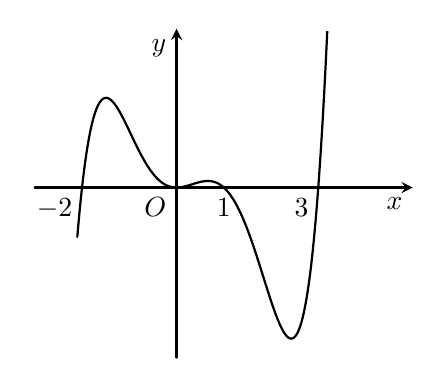
\begin{tikzpicture}[line join=round, line cap=round,>=stealth,thick, scale=.6,yscale=.6]
			\draw[->] (-3,0)--(5,0) node[below left] {$x$};
			\draw[->] (0,-6)--(0,5.6) node[below left] {$y$};
			\draw (0,0) node [below left] {$O$};
			\foreach \x/\nx in {1/1}
			\draw[thin] (\x,1pt)--(\x,-1pt) node [below] {$\nx$};
			\foreach \x/\nx in {-2/-2,3/3}
			\draw[thin] (\x,1pt)--(\x,-1pt) node [below left] {$\nx$};
			%	\foreach \y/\ny in {1/1}
			%	\draw[thin] (1pt,\y)--(-1pt,\y) node [above right] {$\ny$};
			%	\foreach \y/\ny in {-1/-1}
			%	\draw[thin] (1pt,\y)--(-1pt,\y) node [right] {$\ny$};
			%\draw[dashed,thin] (-0.99,-4.5)--(-0.99,4.5);
			\begin{scope}
				\clip (-2.5,-5.5) rectangle (3.5,5.5);
				\draw[samples=200,domain=-2.1:3.2,smooth,variable=\x] plot(\x,{1.0/4.0*((\x)+2.0)*(\x)^(2.0)*((\x)-1.0)*((\x)-3.0)});
				%\draw[dashed,thin] (-4.5,1/1)--(4.5,1/1);
			\end{scope}
	\end{tikzpicture}}
	\loigiai{
		Từ đồ thị của hàm số $y=f'(x)$ ta có bảng biến thiên của hàm số $y=f(x)$ như sau
		\begin{center}
			
\begin{tikzpicture}
				\tkzTabInit[nocadre=true,lgt=1.2,espcl=2.5,deltacl=0.5]
				{$x$ /0.75, $y'$/0.75, $y$/2}
				{$ -\infty $,$-2$,$0$,$ 1 $,$ 3 $,$+\infty $}
				%dòng xét dấu
				\tkzTabLine{,-,0,+,0,+,0 ,-, 0,+,} 
				\tkzTabVar{+/,-/,R,+/,-/,+/} 
			\end{tikzpicture}
		\end{center}			
		Từ bảng biến thiên ta có
		\begin{itemchoice}
			\itemch 
			Bảng biến thiên có $y'$ đổi dấu qua $3$ giá trị nên hàm số $y=f(x)$ có ba điểm cực trị.
			\itemch 
			Hàm số $y=f(x)$ nghịch biến trên khoảng $(-\infty; -2)$.
			\itemch 
			Ta có $g'(x)=2xf'\left(x^2\right)=0\Leftrightarrow \hoac{&x=0	\\&x^2=0\\&x^2=1\\&x^2=3 }\Leftrightarrow \hoac{&x=0	\\&x=\pm 1\\&x=\pm 3.}$\\
			Bảng xét dấu của $g'(x)$
			\begin{center}
				
\begin{tikzpicture}[scale=.8]	\tkzTabInit[deltacl=0.5,espcl=2.5,lgt=2,nocadre]
					{$x$/1,$g'(x)$/1}
					{$-\infty$,$-\sqrt{3}$,$-1$,$0$,$1$,$\sqrt{3}$,$+\infty$}
					\tkzTabLine{,-,$0$,+,$0$,-,$0$,+,$0$,-,$0$,+,}
				\end{tikzpicture}
			\end{center}
			Từ bảng xét dấu của $g'(x)$ ta thấy hàm số $g(x)$ đồng biến trên khoảng $\left(\sqrt{3};+\infty\right)$ nên hàm số $g(x)$ cũng đồng biến trên khoảng $\left(\sqrt{5};+\infty\right)$.
			\itemch 
			Từ bảng xét dấu của $g'(x)$ ta thấy $g'(x)$ đổi dấu $5$ lần nên hàm số $g(x)=f\left(x^2\right)$ có $5$ điểm cực trị.
		\end{itemchoice}		
	}
\end{ex}




\Closesolutionfile{ans}

\ind{PHẦN III.} \inden{Câu trả lời ngắn.}\\
\setcounter{ex}{0}
\Opensolutionfile{ans}[ans/2D1-Bai1-TLN]%--Đặt tên 2D1-Bai1-DS


\begin{ex}%[2D1V1-3]
	[Trích đề thi GHKI -Lớp 12 -THPT-Tam Phú-Năm học 2024-2025]
	Cho hàm số $y=-x^3+3x^2+(m+2)x-2024$. Tính tổng các giá trị nguyên của tham số $m \in \left[-10;5\right]$ để hàm số  nghịch biến trên $\mathbb{R}$.
	\shortans{$-45$}
	\loigiai{
		Tập xác định $\mathscr{D}=\mathbb{R}$ và có đạo hàm
		$$
		y'=-3x^2+6x+m+2.
		$$
		Hàm số nghịch biến trên $\mathbb{R}$ khi và chỉ khi
		$$
		-3x^2+6x+m+2 \le 0, \quad \forall x \in \mathbb{R}
		$$
		Điều này xảy ra khi
		\begin{align*}
			\Delta'=(3)^2-(-3)(m+2) &\le 0 \\
			3m+15 &\le 0 \\
			m &\le -5.
		\end{align*}
		Với điều kiện $m$ nhận các giá trị nguyên và $m \in \left[-10;5\right]$ thì
		$$
		m \in \{ -10; -9; \ldots ; -5 \}.
		$$
		Tổng các giá trị này của $m$ là
		$$
		(-10)+(-9)+\cdots+(-5)= -45.
		$$
	}
\end{ex}
\begin{ex}%[2D1V2-3]
	[Trích đề thi HKI -Lớp 12-THPT Chuyên Trần Phú-Hải Phòng -Năm học 2024-2025]
	Cho hàm số $y =-18x^3+9\left(m^2+1\right)x^2+6(2-3m)x+2019$ với $m$ là tham số thực. Tìm giá trị của $m$ để hàm số đạt cực tiểu tại $x =\dfrac{1}{3}$.
	\shortans[]{$2$}
	\loigiai{
		Ta có $y' =-54x^2+18\left(m^2+1\right)x+6(2-3m)$.\\
		Suy ra $y''=-108x+18\left(m^2+1\right)$.\\
		Do hàm số đạt cực tiểu tại $x =\dfrac{1}{3}$ nên
		\allowdisplaybreaks
		\begin{eqnarray*}
			\heva{&y'\left(\dfrac{1}{3}\right)=0\\&y''\left(\dfrac{1}{3}\right)>0}
			&\Rightarrow & \heva{& -6+6(m^2+1) -18m+12= 0\\&-36+18(m^2+1)>0}\\
			&\Rightarrow & \heva{& \hoac{&m =1\\&m=2}\\&m^2>1}\\
			&\Rightarrow & m=2.
		\end{eqnarray*}
	}
\end{ex}
\begin{ex}%[2D1V1-1]
	[Trích đề thi HK1-lớp 12-SGD-Tỉnh Vĩnh Long-Năm học-2024-2025]
	Một chất điểm chuyển động có phương trình $s(t)$ thì có vận tốc $v(t)=s'(t)$. Biết rằng phương trình chuyển động của chất điểm là $s(t)=\dfrac{1}{3}t^3-3t^2+5t$ trong đó $t$ được tính bằng giây và $s$ được tính bằng mét. Kể từ giây thứ bao nhiêu trở đi thì vận tốc của chất điểm bắt đầu tăng?
	\shortans{3}
	\loigiai{
		Ta có $v(t)=s'(t)=t^2-6t+5$, $t \ge 0$, suy ra $v'(t)=2t-6$.\\
		Lại có $v'(t)=0 \Leftrightarrow t=3$.\\
		Bảng biến thiên
		\begin{center}
			
\begin{tikzpicture}
				\tkzTabInit[nocadre=true,lgt=1.2,espcl=3,deltacl=0.5]
				{$t$ /.7,$v'(t)$ /0.7,$v(t)$ /2}
				{$0$, $3$, $+ \infty$}
				\tkzTabLine{,-,0,+,}
				\tkzTabVar{+/$+ \infty$ ,-/$-4$,+/$+ \infty$}
			\end{tikzpicture}
		\end{center}
		Kể từ giây thứ $3$ trở đi thì vận tốc của chất điểm bắt đầu tăng.
	}
\end{ex}

\begin{ex}%[2D1V2-2]
	[Trích đề thi GHK1-Lớp 12 -THPT-HungVuong-TpHCM-Năm học 2024-2025]
	Cho hàm số $y=f(x)$ xác định và liên tục trên $\mathbb{R}$. Hàm số $y=f'(x)$ có đồ thị như hình vẽ sau.
	\begin{center}
		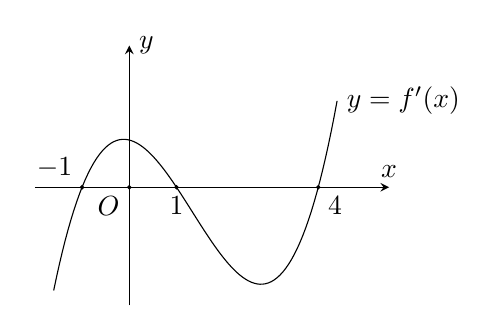
\begin{tikzpicture}[>=stealth, scale=.6]
			\draw[->](-2,0)--(0,0) node[below left]{$O$} --(5.5,0) node[above]{$x$};
			\draw[->](0,-2.5)--(0,3) node[right]{$y$};
			\draw plot [domain=-1.6:4.4, samples=100] (\x, {0.25*(\x)^3-1*(\x)^2-0.25*\x+1}) node[right] {$y=f'(x)$};
			\draw[fill=black](-1,0) node[above left]{$-1$} circle (1pt);
			\draw[fill=black](1,0) node[below]{$1$} circle (1pt);
			\draw[fill=black](4,0) node[below right]{$4$} circle (1pt);
			\draw[fill=black](0,0) circle (1pt);
		\end{tikzpicture}
	\end{center}
	Hàm số $y=f(x^2-1)$ có bao nhiêu điểm cực trị?
		\shortans{5}
	\loigiai{
		Ta có $y'=2x\cdot f'(x^2-1)$.\\
		$y'=0 \Leftrightarrow \hoac{&x=0\\&f'(x^2-1)=0}\Leftrightarrow \hoac{&x=0\\&x^2-1=-1\\&x^2-1=1\\&x^2-1=4}\Leftrightarrow \hoac{&x=0\\&x=\pm \sqrt{2}\\&x=\pm \sqrt{5}.}$\\
		Bảng biến thiên của hàm số $y=f(x)$ như sau
		\begin{center}
			
\begin{tikzpicture}
				\tkzTabInit[nocadre=true,lgt=1,espcl=2]{$x$/0.6,$y'$/0.6,$y$/2}{$-\infty$,$-\sqrt{5}$,$-\sqrt{2}$,$0$,$\sqrt{2}$,$\sqrt{5}$,$+\infty$}
				\tkzTabLine{,-,$0$,+,$0$,-,$0$,+,$0$,-,$0$,+}
				\tkzTabVar{+/$+\infty$,-/$f(4)$,+/$f(1)$,-/$f(-1)$,+/$f(1)$,-/$f(4)$,+/$+\infty$}
			\end{tikzpicture}
		\end{center}
		Vậy hàm số có $5$ điểm cực trị.
	}
\end{ex}
\begin{ex}%[2D1C1-5]
	[Trích đề thi HKI-lớp 12-THPT CHUYÊN HẠ LONG- QUẢNG NINH-Năm học-2024-2025]
	\immini{Cho điểm $A$ di động trên nửa đường tròn tâm $O$ đường kính $MN=20$\,cm, $\widehat{MOA}=\alpha$ ($0 < \alpha < \pi$). Lấy điểm $B$ thuộc nửa đường tròn và $C, D$ thuộc đường kính $MN$ sao cho $ABCD$ là hình chữ nhật. Khi $A$ di động từ trái sang phải, khi đó trong các khoảng $(a;b]$ và $[c;d]$ của $\alpha$ thì diện tích của hình chữ nhật $ABCD$ tăng. Tính $a+b+c+d$ (kết quả làm tròn đến hàng phần trăm).}{\begin{tikzpicture}[>=stealth,line join=round,line cap=round,font=\footnotesize,scale=1] 
			\path
			(0:0) coordinate (O)
			(180:3) coordinate (M)
			(0:3) coordinate (N)
			(150:3) coordinate (A)
			(30:3) coordinate (B)
			(90:3) coordinate (H)
			($(M)!(A)!(N)$) coordinate (D)
			($(M)!(B)!(N)$) coordinate (C);
			\draw (180:3) arc (180:0:3); 
			\draw (M)--(N)(D)--(A)--(B)--(C)
			(A)--(O);
			\draw[dashed](O)--(H);
			\foreach \x/\y/\z in {B/A/D,A/B/C,B/C/D,C/D/A}{
				\path (\y) pic[draw,angle radius=5pt]{right angle=\x--\y--\z};}
			\foreach \x/\y/\z in {A/O/D}{
				\path (\y) pic[draw,angle radius=8pt,angle eccentricity=1.5,"$\alpha$"]{angle=\x--\y--\z};}
			\path (M)--(N)--([turn]-90:12pt) coordinate (xt)
			($(M)-(N)+(xt)$) coordinate (yt);
			\draw[>=stealth,|<->|] (xt)--(yt) node[fill=white,inner sep=0pt,font=\scriptsize,pos=0.5,sloped]{$20\mathrm{~cm}$};
			\foreach \t/\goc in {O/-90, M/180,N/0,A/120,B/60,C/-90,D/-90}{
				\draw[fill=black] (\t) circle (1pt) node[font=\scriptsize,shift={(\goc:5pt)}] {$\t$};
			}
	\end{tikzpicture}}
	\shortans{$4{,}71$}
	\loigiai{
		Gọi R là bán kính đường tròn, ta có ${R=\dfrac{MN}{2}=\dfrac{20}{2}=10 cm}$.\\
		Trong tam giác vuông $ADO$, ta có:\\
		${OD =\cos \alpha=R \cos \alpha=10 \cos \alpha}$\\
		${AD =\sin \alpha=R \sin \alpha=10 \sin \alpha}$.\\
		Suy ra ${CD=2OD=2 \cdot 10 \cos \alpha=20 \cos \alpha}$.\\
		Diện tích hình chữ nhật $ABCD$ là\\
		${S(\alpha)=AD \cdot CD=(10 \sin \alpha) \cdot (20 \cos \alpha)=200 \sin \alpha \cos \alpha=100 \sin(2\alpha)}$.\\
		Để diện tích hình chữ nhật tăng, ta cần ${S' (\alpha) \ge 0}$.\\
		${S'(\alpha)=100 \cdot \cos(2\alpha)=200 \cos(2\alpha)}$.\\
		${S' (\alpha) \ge 0 \Leftrightarrow 200 \cos(2\alpha) > 0 \Leftrightarrow \cos(2\alpha) \ge 0}$.
		\begin{itemize}
			\item Với $0 < \alpha < \dfrac{\pi}{2}$, ta có $0 < 2\alpha < \pi$.\\
			Suy ra $\cos(2\alpha) \ge 0$ khi $\alpha \in \left(0;\dfrac{\pi}{4}\right]$.
			\item Với $\dfrac{\pi}{2} < \alpha < \pi$, ta có $0 < \pi -\alpha< \dfrac{\pi}{2}$.\\
			Diện tích hình chữ nhật $ABCD$ là $100\sin2(\pi-\alpha)$.\\
			$S'(\alpha)=-100 \cdot \cos2(\pi-\alpha)=-200 \cos2(\pi-\alpha)$.\\
			Suy ra 	$S' (\alpha) \ge 0$ khi $\alpha \in \left[ \dfrac{\pi}{2};   \dfrac{3\pi}{4}\right]$.
		\end{itemize}
		Vậy các khoảng cần tìm là $\left(a;b\right]=\left(0;\dfrac{\pi}{4}\right]$ và $[c;d]=\left[ \dfrac{\pi}{2};   \dfrac{3\pi}{4}\right]$.\\
		$a=0$, $b=\dfrac{\pi}{4}$, $c=\dfrac{\pi}{2}$, $d=\dfrac{3\pi}{4}$.\\
		Vậy	${a+b+c+d=0+\dfrac{\pi}{4}+\dfrac{\pi}{2}+ \dfrac{3\pi}{4}\approx 4{,}71}$.
	}
\end{ex}

\Closesolutionfile{ans}

\ind{PHẦN IV.} \inden{Tự luận.}\\
\setcounter{ex}{0}
\begin{ex}%[2D1N1-1]
	[Trích đề thi HKI -Lớp 12 -SGD-HUẾ -Năm học 2024-2025]
	Tìm các khoảng đơn điệu của hàm số $y=x^3-3x+1$.
	\loigiai{
		Tập xác định $\mathscr{D}=\mathbb{R}$.\\
		Đạo hàm $y'=3x^2-3$.\\
		Cho $y'=0 \Leftrightarrow 3x^2-3=0 \Leftrightarrow x^2=1 \Leftrightarrow x=\pm 1$.\\
	Bảng biến thiên
		\begin{center}
			
\begin{tikzpicture}
				\tkzTabInit[nocadre=true,lgt=1,espcl=2.5,deltacl=0.5]
				{$x$/.7 ,$y'$/.7,$y$/2}
				{$-\infty$ , $-1$ , $1$ , $+\infty$}
				\tkzTabLine{ ,+, $0$ ,-, $0$ ,+, }
				\tkzTabVar{-/$-\infty$ ,+/$ $ , -/$ $ ,+/$+\infty$}
			\end{tikzpicture}
		\end{center}
		Từ bảng biến thiên, ta có
		\begin{itemize}
			\item Hàm số đồng biến trên các khoảng $(-\infty; -1)$ và $(1;+\infty)$.
			\item Hàm số nghịch biến trên khoảng $(-1; 1)$.
		\end{itemize}
	}
\end{ex}
\begin{ex}%[2D1H1-1]
	Xét tính đơn điệu của hàm số $y=\dfrac{x^2+x+4}{x+1}$.
	\loigiai{
		Tập xác định $\mathscr{D}=\mathbb{R}\setminus\left\{-1\right\}$.\\
		Đạo hàm $y'=\dfrac{x^2+2x-3}{\left(x+1\right)^2}$.\\
		$y'=0\Rightarrow\hoac{& x=1\Rightarrow y=3 \\ & x=-3\Rightarrow y=-5.}$\\
		Bảng biến thiên\\
		\centerline{
			
\begin{tikzpicture}
				\tkzTabInit[nocadre=true,lgt=1,espcl=2.5,deltacl=0.5]{$x$/.7 ,$y'$/.7,$y$/2}
				{$-\infty$ , $-3$ , $-1$ , $1$ , $+\infty$}
				\tkzTabLine{ ,+, $0$ ,-, d ,-, $0$ ,+, }
				\tkzTabVar{-/$-\infty$ ,+/$-5$ , -D+/$-\infty$/$+\infty$ , -/$3$ ,+/$+\infty$}
			\end{tikzpicture}
		}
		Hàm số đồng biến trên khoảng $\left(-\infty;-3\right)$ và $\left(1;+\infty\right)$.\\
		Hàm số nghịch biến trên khoảng $\left(-3;-1\right)$ và $\left(-1;1\right)$.
	}
\end{ex}
\begin{ex}%[2D1H1-5]
	[Trích đề ôn tập HKI -Lớp 12 -THPT Bùi Thị Xuân-Năm học 2024-2025]
	Một vật đang đứng yên thì bắt đầu chuyển động theo quy luật $s(t)=-t^3+3t^2+6t$, với $t$ (giây) là khoảng thời gian tính từ lúc vật bắt đầu chuyển động và $s$ (mét) là quãng đường vật đi được trong khoảng thời gian đó. Hỏi vật tăng tốc trong khoảng thời gian bao nhiêu giây tính từ lúc bắt đầu chuyển động?
	\loigiai{Vận tốc của vật là $v(t)=s'(t)=-3t^2+6t+6$.\\
		Ta có $v'(t)=-6t+6$.\\
		Cho $v'(t)=0 \Leftrightarrow t=1$.\\
		Bảng biến thiên\\
		\begin{center}
			
\begin{tikzpicture}
				\tkzTabInit[nocadre=true,lgt=1.2,espcl=2.5,deltacl=0.6]
				{$t$/0.6,$v'(t)$/0.6,$v(t)$/2}{$0$,$1$,$+\infty$}
				\tkzTabLine{,+,0,-,}
				\tkzTabVar{-/$6$,+/$9$,-/$-\infty$}
			\end{tikzpicture}
		\end{center}
		Dựa vào bảng biến thiên, ta thấy $v(t)$ tăng khi $t\in (0;1)$. Vậy vật tăng tốc trong khoảng thời gian từ gian $1$ giây tính từ lúc bắt đầu chuyển động.
	}
\end{ex}
\begin{ex}%[2D1V1-1]
	[Trích đề thi HKI -Lớp 12 -SGD-Tỉnh Vĩnh Long-Năm học 2024-2025]
	Một chất điểm chuyển động có phương trình $s(t)$ thì có vận tốc $v(t)=s'(t)$. Biết rằng phương trình chuyển động của chất điểm là $s(t)=\dfrac{1}{3}t^3-3t^2+5t$ trong đó $t$ được tính bằng giây và $s$ được tính bằng mét. Kể từ giây thứ bao nhiêu trở đi thì vận tốc của chất điểm bắt đầu tăng?
	\loigiai{
		Ta có $v(t)=s'(t)=t^2-6t+5$, $t \ge 0$, suy ra $v'(t)=2t-6$.\\
		Lại có $v'(t)=0 \Leftrightarrow t=3$.\\
		Bảng biến thiên
		\begin{center}
			
\begin{tikzpicture}
				\tkzTabInit[nocadre=true,lgt=1.2,espcl=2.5,deltacl=0.8]
				{$x$ /1,$v'$ /0.6,$v$ /2}
				{$0$, $3$, $+ \infty$}
				\tkzTabLine{,-,0,+,}
				\tkzTabVar{+/$+ \infty$ ,-/$-4$,+/$+ \infty$}
			\end{tikzpicture}
		\end{center}
		Kể từ giây thứ $3$ trở đi thì vận tốc của chất điểm bắt đầu tăng.
	}
\end{ex}
\begin{ex}%[2D1H3-1]
	[Trích đề thi GHKI -Lớp 12 -THPT Phạm Văn Sáng-Tp HCM-Năm học 2024-2025]
	Người ta giới thiệu một loại thuốc để kích thích sự sinh sản của một loại vi khuẩn. Sau $t$ phút, số lượng vi khuẩn được xác định theo công thức là $f(t)=-t^3+30t^2+1\,000$ với $0\leq t\leq 30$. Hỏi sau bao nhiêu phút thí số lượng vi khuẩn đạt giá trị cực đại?
	\loigiai{
		Xét hàm số $f(t)=-t^3+30t^2+1\,000$ trên đoạn $[0;30]$.\\
		Ta có $f'(t)=-3t^2+60t$; $f'(t)=0\Leftrightarrow -3t^2+60t=0\Leftrightarrow\hoac{&t=0\in[0;30]\\&t=20\in[0;30].}$\\
		Mà $f(0)=1\,000$; $f(20)=5\,000$; $f(30)=1\,000$.\\
		Vậy $\max\limits_{[0;30]}f(t)=f(20)=5\,000$ hay số lượng vi khuẩn đạt giá trị cực đại là $5\,000$ sau $20$ phút.
	}
\end{ex}
\begin{ex}%[2D1V1-3]
	[Lớp 12 – Đề thi học kì 1]
	Có tất cả bao nhiêu giá trị nguyên của tham số $m$ thuộc đoạn $[-24;24]$ để hàm số $y=\dfrac{(m+1)x+m}{2x+1}$ đồng biến trên từng khoảng xác định của nó?
	\loigiai{Tập xác định $\mathscr{D}=\mathbb{R}\setminus \left\{ -\dfrac{1}{2} \right\}$.\\
		Ta có $y'=\dfrac{1-m}{\left( 2x+1 \right)^2}$.\\
		Hàm số đồng biến trên từng khoảng xác định
		\allowdisplaybreaks
		\begin{eqnarray*}
			& &y'>0,\, \forall x\in \mathscr{D}\\
			&\Leftrightarrow &\dfrac{1-m}{\left( 2x+1 \right)^2} >0,\, \forall x\in \mathscr{D}\\
			&\Leftrightarrow &1-m>0\\
			&\Leftrightarrow &m<1.
		\end{eqnarray*}
		Mà $m\in \mathbb{Z}$ và $m\in [-24;24]$ nên $m\in \left\{ -24;-23;\ldots;0 \right\}$.\\
		Vậy có $25$ giá trị nguyên của tham số $m$ thỏa đề.}
\end{ex}
\begin{ex}%[2D1V1-5]
	[Trích đề thi HKI -Lớp 12 -SGD-HUẾ-Năm học 2024-2025]
	Một chất điểm đang chuyển động trên một đường thẳng và gặp một con dốc cao muốn vượt qua. Xem chân dốc là điểm $A$, khi chất điểm qua $A$ là thời điểm bắt đầu leo dốc với phương trình chuyển động là $s(t)=at-2t^2$ cho đến khi lên đỉnh dốc ($a$ là tham số thực dương, $t \geq 0$ tính bằng giây và $s$ tính bằng mét). Biết dốc có độ dài bằng $50m$ và xe muốn leo dốc thành công thì phải tồn tại $t > 0$ sao cho $s(t)=50$. Tính vận tốc ban đầu nhỏ nhất để xe leo dốc thành công.
	\loigiai{
		Ta có phương trình chuyển động của chất điểm $s(t)=at-2t^2$.\\
		Để xe leo dốc thành công thì phải tồn tại $t > 0$ sao cho $s(t)=50$, hay $at-2t^2=50$ hay $2t^2-at+50=0$.\\
		Để phương trình trên có nghiệm $t > 0$ thì trước hết $\Delta \geq 0$, tức là $$(-a)^2-4.2.50 \geq 0 \Leftrightarrow a^2 \geq 400 \Leftrightarrow a \geq 20 \left(\text{ do } a>0\right).$$
		Gọi $t_1, t_2$ là hai nghiệm của phương trình $2t^2-at+50=0$. Theo định lý Viète, ta có
		$$\heva{&t_1+t_2=\dfrac{a}{2}\\&t_1 t_2=\dfrac{50}{2}=25.}$$
		Để tồn tại nghiệm $t>0$, ta có $2$ trường hợp xảy ra
		\begin{itemize}
			\item  Cả $2$ nghiệm đều dương $\Leftrightarrow t_1+t_2 > 0$ và $t_1t_2 >0$ (đã thoả mãn).
			\item Có $1$ nghiệm dương và 1 nghiệm âm. Lúc này ta có $t_1t_2<0$. Điều này mâu thuẫn với $t_1t_2=25>0$, vậy trường hợp này không xảy ra.
		\end{itemize}
		Vậy điều kiện để phương trình có nghiệm dương là  $\Delta \geq 0 \Leftrightarrow a\geq 20$.\\
		Vận tốc của chất điểm là $v(t)=s'(t)=a-4t$. Vận tốc ban đầu ứng với $t=0$ là $v(0)=a$.\\
		Để xe leo dốc thành công thì phương trình $at-2t^2=50$ phải có nghiệm dương, tức là $a \geq 20$.\\
		Vậy vận tốc ban đầu nhỏ nhất để xe leo dốc thành công là $20$ m/s.
	}
\end{ex}

\begin{ex}%[2D1V2-1]
	[Trích đề thi HKI -Lớp 12 -THPT Đinh Tiên Hoàng-Tỉnh Ninh Bình-Năm học 2024-2025]
	Cho hàm số $y=f(x)$ có đạo hàm $f'(x)=\left(x^2-x\right)\left(x^2-4x+3\right)$, $\forall x \in \mathbb{R}$. Tính tổng tất cả các giá trị nguyên của tham số $m$ để hàm số $g(x)=f\left(x^2+m\right)$ có $3$ điểm cực trị.
	\loigiai{
		Ta có $f'(x)=x(x-3)(x-1)^2$.\\
		Ta có $g'(x)=2xf'(x^2+m)=2x(x^2+m)(x^2+m-3)(x^2+m-1)^2$.\\
		Do đó $g'(x)=0$ có ba điểm cực trị khi phương trình $g'(x)=0$ có $3$ nghiệm bội lẻ phân biệt.\\
		Hay $\hoac{&x^2=-m\\&x^2=-m+3}$ có $2$ nghiệm thực phân biệt $ \Leftrightarrow 0 \le m < 3 $.\\
		Vậy tổng tất cả các giá trị nguyên của tham số $m$ để hàm số $g(x)$ có $3$ điểm cực trị là $0+1+2=3$.
	}
\end{ex}
\begin{ex}%[2D1H2-7]
	[Trích đề thi  HKI Lớp 12-THPT Thực hành Sư Phạm-Đồng Nai-Năm học 2024-2025]
	Đường ray của tàu lượn siêu tốc là một dạng đường cong Spline được thiết kế với độ cong thay đổi linh hoạt, thú vị và đáp ứng được một số tiêu chí về an toàn.
	\begin{flushright}
		(Nguồn: J.R.McKilligan \& T.J.Allen. The Mathematics of Coaster Design)
	\end{flushright} 
	Một phần đường ray tàu lượn siêu tốc có dạng đồ thị hàm số bậc ba
	\[y=f(x)=a x^3+b x^2+c x+d,(a \neq 0)\]
	Trục $Ox$ mô tả quãng đường tàu di chuyển theo chiều ngang (tính bằng mét), trục $Oy$ mô tả chiều cao của đường ray (tính bằng mét) tại mỗi vị trí $x$. Chiều cao xuất phát là $50$ m. Tàu xuống dưới mặt đất lần thứ nhất từ vị trí $x=20$ m, tàu lên khỏi mặt đất ở vị trí $x=50$ m và sau đó xuống dưới mặt đất lần thứ hai ở vị trí $x=100$ m. Xét đồ thị của hàm số đã cho khi $x \in[0; 100]$ như hình vẽ bên dưới
	\begin{center}
		\begin{tikzpicture}[>=stealth,scale=0.07]
			\def\xmin{-5};\def\xmax{105};\def\ymin{-10};\def\ymax{60};
			\draw[->] (\xmin,0)--(\xmax,0) node[below right] {$x$};
			\draw[->] (0,\ymin)--(0,\ymax) node[above left] {$y$};
			\draw (0,0) node [below left] {$O$};
			\begin{scope}
				\clip (\xmin,\ymin) rectangle (\xmax,\ymax);
				\draw[samples=200,domain=\xmin:\xmax,smooth,variable=\x] plot (\x,{(-1/2000)*(\x-20)*(\x-50)*(\x-100)});
			\end{scope}
			\draw[fill=black]
			(20,0) circle(5pt)node[below]{$20$}	
			(50,0) circle(5pt)node[below]{$50$}	
			(100,0) circle(5pt)node[below left]{$100$}
			(0,50) circle(5pt)node[left]{$50$}	
			; 
		\end{tikzpicture}
	\end{center}
	Biết điểm cao nhất của đường ray khi tàu lên khỏi mặt đất và điểm thấp nhất của đường ray khi tàu xuống dưới mặt đất lần lượt có hoành độ là $p$ và $q$. Tính $3q+p$.
	\loigiai{
		Đồ thị giao với trục hoành tại các điểm $(20;0)$; $(50;0)$; $(100;0)$.\\
		Suy ra phương trình $f(x)=0$ có ba nghiệm $x=20$; $x=50$; $x=100$.\\
		Nên $f(x)$ có dạng $f(x)=a\cdot(x-20)(x-50)(x-100)$.\\
		Do $f(0)=50$, suy ra $a=-\dfrac{1}{2000}$.\\
		Suy ra $y=-\dfrac{1}{2000}(x-20)(x-50)(x-100)=-\dfrac{1}{2000} x^3+\dfrac{17}{200} x^2-4 x+50$.\\
		Các điểm cần tìm chính là các điểm cực trị của hàm số $y=f(x)$.\\
		Ta có $y'=-\dfrac{3}{2000} x^2+\dfrac{34}{200} x-4=0 \Leftrightarrow\hoac{&x=\dfrac{100}{3}\Rightarrow y=-\dfrac{200}{27} \\& x=80\Rightarrow y=18.}$\\
		Lập bảng biến thiên
		\begin{center}
			\begin{tikzpicture}
				\tkzTabInit[nocadre,lgt=1.4,espcl=2.2,deltacl=0.5]{$x$/.7 ,$f'(x)$/.7,$f(x)$/2}
				{$-\infty$ , $\tfrac{100}{3}$ , $80$ , $+\infty$}
				\tkzTabLine{ ,-, $0$ ,+, $0$ ,-, }
				\tkzTabVar{+/$+\infty$ , -/$-\dfrac{200}{27}$ ,+/$18$ , -/$-\infty$}
			\end{tikzpicture}
		\end{center}
		Ta được $A\left(\dfrac{100}{3} ;-\dfrac{200}{27}\right)$ và $B(80;18)$ lần lượt là điểm cục tiểu và điểm cực đại của đồ thị hàm số $y=f(x)$.\\ 
		Do đó $q=\dfrac{100}{3}$; $p=80 \Rightarrow 3 q+p=180$.	
	}
\end{ex}
\begin{ex}%[2D1V1-4]
	[Trích đề thi GHKI -Lớp 12 -THPT Chuyên Lê Khiết-Quảng Ngãi-Năm học 2024-2025]
	Giả sử doanh số (tính bằng số sản phẩm) của một sản phẩm mới (trong vòng một số năm nhất định) của công ty $A$ tuân theo quy luật logistic được mô hình hóa bẳng hàm số $R=R(t)=\dfrac{a}{1+b \mathrm{e}^{-t}}, t \geq 0$, trong đó thời gian $t$ được tính bằng năm, kể từ khi phát hành sản phẩm mới. Khi đó đạo hàm $R'(t)$ biểu thị tốc độ bán hàng. Tại thời điểm $t=0$, công ty $A$ có $1\,000$ sản phẩm và tốc độ bán hàng là $800$ sản phẩm/năm. Tính $a+b$.
	\loigiai{
		Tại thời điểm $t=0$, số lượng sản phẩm là $1\,000$ . Do đó		
		$$
		R(0)=\dfrac{a}{1+b \mathrm{e}^{-0}}=\dfrac{a}{1+b}=1\,000.
		$$
		Suy ra	$\dfrac{a}{1+b}=1000$.\qquad (1)\\
		Hàm doanh số $R(t)=\dfrac{a}{1+b \mathrm{e}^{-t}}$ có đạo hàm là
		$$
		R'(t)=\dfrac{a b \mathrm{e}^{-t}}{\left(1+b \mathrm{e}^{-t}\right)^2}.
		$$
		Tại thời điểm $t=0$, tốc độ bán hàng là $800$ sản phẩm/năm. Do đó		
		$$
		R'(0)=\dfrac{a b \mathrm{e}^0}{\left(1+b \mathrm{e}^0\right)^2}=\dfrac{a b}{(1+b)^2}=800.
		$$
		Suy ra $\dfrac{a b}{(1+b)^2}=800$.\qquad (2)\\
		Từ $(1)$ và $(2)$, ta có hệ $\heva{&\dfrac{a}{1+b}=1\,000\\&\dfrac{a b}{(1+b)^2}=800.}$\\
		Giải hệ ta được $a=5\,000$ và $b=4$. \\
		Do đó $a+b=5\,004$.
	}
\end{ex}